\documentclass[10pt]{article}
\usepackage[utf8]{inputenc}
\usepackage[T1]{fontenc}
\usepackage{lmodern}
\usepackage[margin=2cm]{geometry}
\usepackage{graphicx}
\usepackage{booktabs}
\usepackage{adjustbox}
\usepackage{array}
\usepackage[table]{xcolor}
\usepackage{fvextra}
\usepackage{enumitem}
\usepackage[hidelinks]{hyperref}
\setlist{itemsep=2pt}
\setlength{\parindent}{0pt}
\setlength{\parskip}{5pt}
\renewcommand{\arraystretch}{1.15}
% Generated by make_overleaf.py from the results page; edit the generator, not this file.

\begin{document}
\title{Social Knowledge for Cross-Domain User Preference Modeling\\[4pt]\large Reproduction \& extension \textperiodcentered{} arXiv:2603.10148}
\date{}
\maketitle
\begin{itemize}
  \item Gain on less popular entities: \textbf{+38\%} (ranks 81--100, vs. +22\% on the top 20 for the same users)
  \item Popularity vs. chance, ranks 81--100: \textbf{+0.039} (MAP; social similarity is +0.151)
\end{itemize}
\section{Reproduction}
11,153 users who follow more than 10 of the 276 candidate entities, 14 categories, link-prediction evaluation with MAP. On average 855 of the accounts a user follows are SocialVec entities. Follow statistics of all 11,153 users: accounts followed: minimum 59, mean 1,973, median 1,554, maximum 5,000; candidate entities followed: minimum 11, mean 40.3, median 35, maximum 170. No user follows more than 5,000 accounts, which looks like a limit of the data collection.

\subsection*{Table 1 \textperiodcentered{} Entity ranking (MAP)}
\begin{center}\begin{adjustbox}{max width=\linewidth}
\begin{tabular}{lrrrrrrrrrr}
\toprule
Category & Users & Entities / user & Random & Popularity & Social \textperiodcentered{} All & $\Delta$ & Social \textperiodcentered{} Sampled & $\Delta$ & All, target removed & $\Delta$ \\
\midrule
Musical artists & 720 & 7.6 & 0.466 & 0.520 & 0.633 & +22\% & 0.591 & +14\% & 0.629 & +21\% \\
News outlets & 844 & 8.2 & 0.491 & 0.581 & 0.692 & +19\% & 0.661 & +14\% & 0.689 & +19\% \\
Comedians & 854 & 6.8 & 0.432 & 0.545 & 0.599 & +10\% & 0.594 & +9\% & 0.596 & +9\% \\
Politicians & 804 & 11.2 & 0.646 & 0.720 & 0.777 & +8\% & 0.755 & +5\% & 0.774 & +7\% \\
TV stations & 819 & 4.5 & 0.331 & 0.469 & 0.618 & +32\% & 0.603 & +28\% & 0.613 & +31\% \\
Actors & 809 & 6.6 & 0.420 & 0.521 & 0.647 & +24\% & 0.602 & +15\% & 0.644 & +24\% \\
TV shows & 773 & 3.9 & 0.305 & 0.365 & 0.635 & +74\% & 0.551 & +51\% & 0.631 & +73\% \\
Sports teams & 691 & 4.3 & 0.322 & 0.349 & 0.510 & +46\% & 0.385 & +10\% & 0.503 & +44\% \\
Journalists & 948 & 10.1 & 0.571 & 0.622 & 0.675 & +9\% & 0.640 & +3\% & 0.672 & +8\% \\
TV hosts & 835 & 1.8 & 0.216 & 0.301 & 0.428 & +42\% & 0.394 & +31\% & 0.423 & +41\% \\
\midrule
Overall & 8,097 &  & 0.420 & 0.499 & 0.621 & +24\% & 0.578 & +16\% & 0.617 & +24\% \\
\bottomrule
\end{tabular}

\end{adjustbox}\end{center}

{\small The 10 categories that also have a ranks 181--200 list (films, food chains, car makers and fashion are left out, so that all results cover the same categories). Random is the expected MAP of a random ranking. $\Delta$ is the gain over popularity. Sampled is the closed-world setting, where profiles use only the experiment's entities from the other 13 categories.}

\subsection*{Figure 1 \textperiodcentered{} How much data is needed?}
Figure 1 uses the full-scale setup of Table 6 (Section 3): all 36,739 user--category pairs (10,039 distinct users) in which a user follows at least one entity ranked 1--20 and one ranked 81--100 in the 9 categories that list 100 entities. As there, every entity known to belong to the target category is removed from the profile.

\begin{itemize}
  \item \textbf{Small profiles are enough.} With k = 50 sampled accounts SocialVec reaches 98.4\% of its full-profile score on the top 20 and 98.7\% at ranks 81--100; both curves level off beyond about 100 accounts.
  \item \textbf{Both bands beat popularity from the smallest profile.} With k = 10 accounts SocialVec scores 0.590 vs. popularity's 0.513 on the top 20 and 0.365 vs. 0.291 at ranks 81--100; the full profiles score 0.633 and 0.400.
\end{itemize}
All values average the 9 categories; the values are in Table 2. The full-profile scores equal Table 6's.

\begin{center}
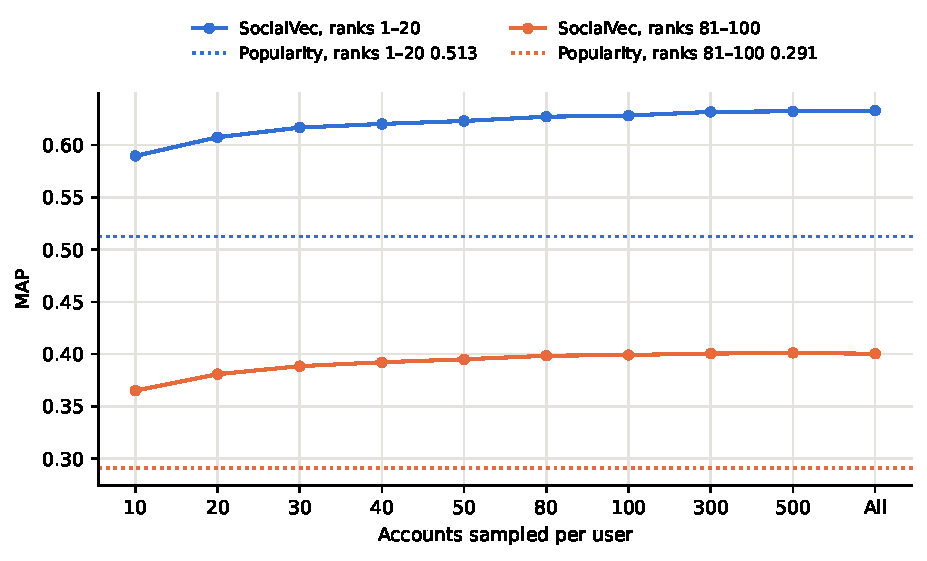
\includegraphics[width=\linewidth,height=0.5\textheight,keepaspectratio]{figures/figure1_overall.pdf}
\end{center}

\subsubsection*{Table 2 \textperiodcentered{} Overall MAP by number of sampled accounts, ranks 1--20 and 81--100 (data of Figure 1)}
\begin{center}\begin{adjustbox}{max width=\linewidth}
\begin{tabular}{lrr}
\toprule
k & Ranks 1--20 & Ranks 81--100 \\
\midrule
10 & 0.590 & 0.365 \\
20 & 0.607 & 0.381 \\
30 & 0.617 & 0.388 \\
40 & 0.620 & 0.392 \\
50 & 0.623 & 0.395 \\
80 & 0.627 & 0.398 \\
100 & 0.628 & 0.399 \\
300 & 0.632 & 0.400 \\
500 & 0.632 & 0.401 \\
5000 & 0.633 & 0.400 \\
\midrule
All & 0.633 & 0.400 \\
Popularity & 0.513 & 0.291 \\
Random (expected) & 0.440 & 0.252 \\
\bottomrule
\end{tabular}

\end{adjustbox}\end{center}

\subsubsection*{Per-category panels}
\begin{center}
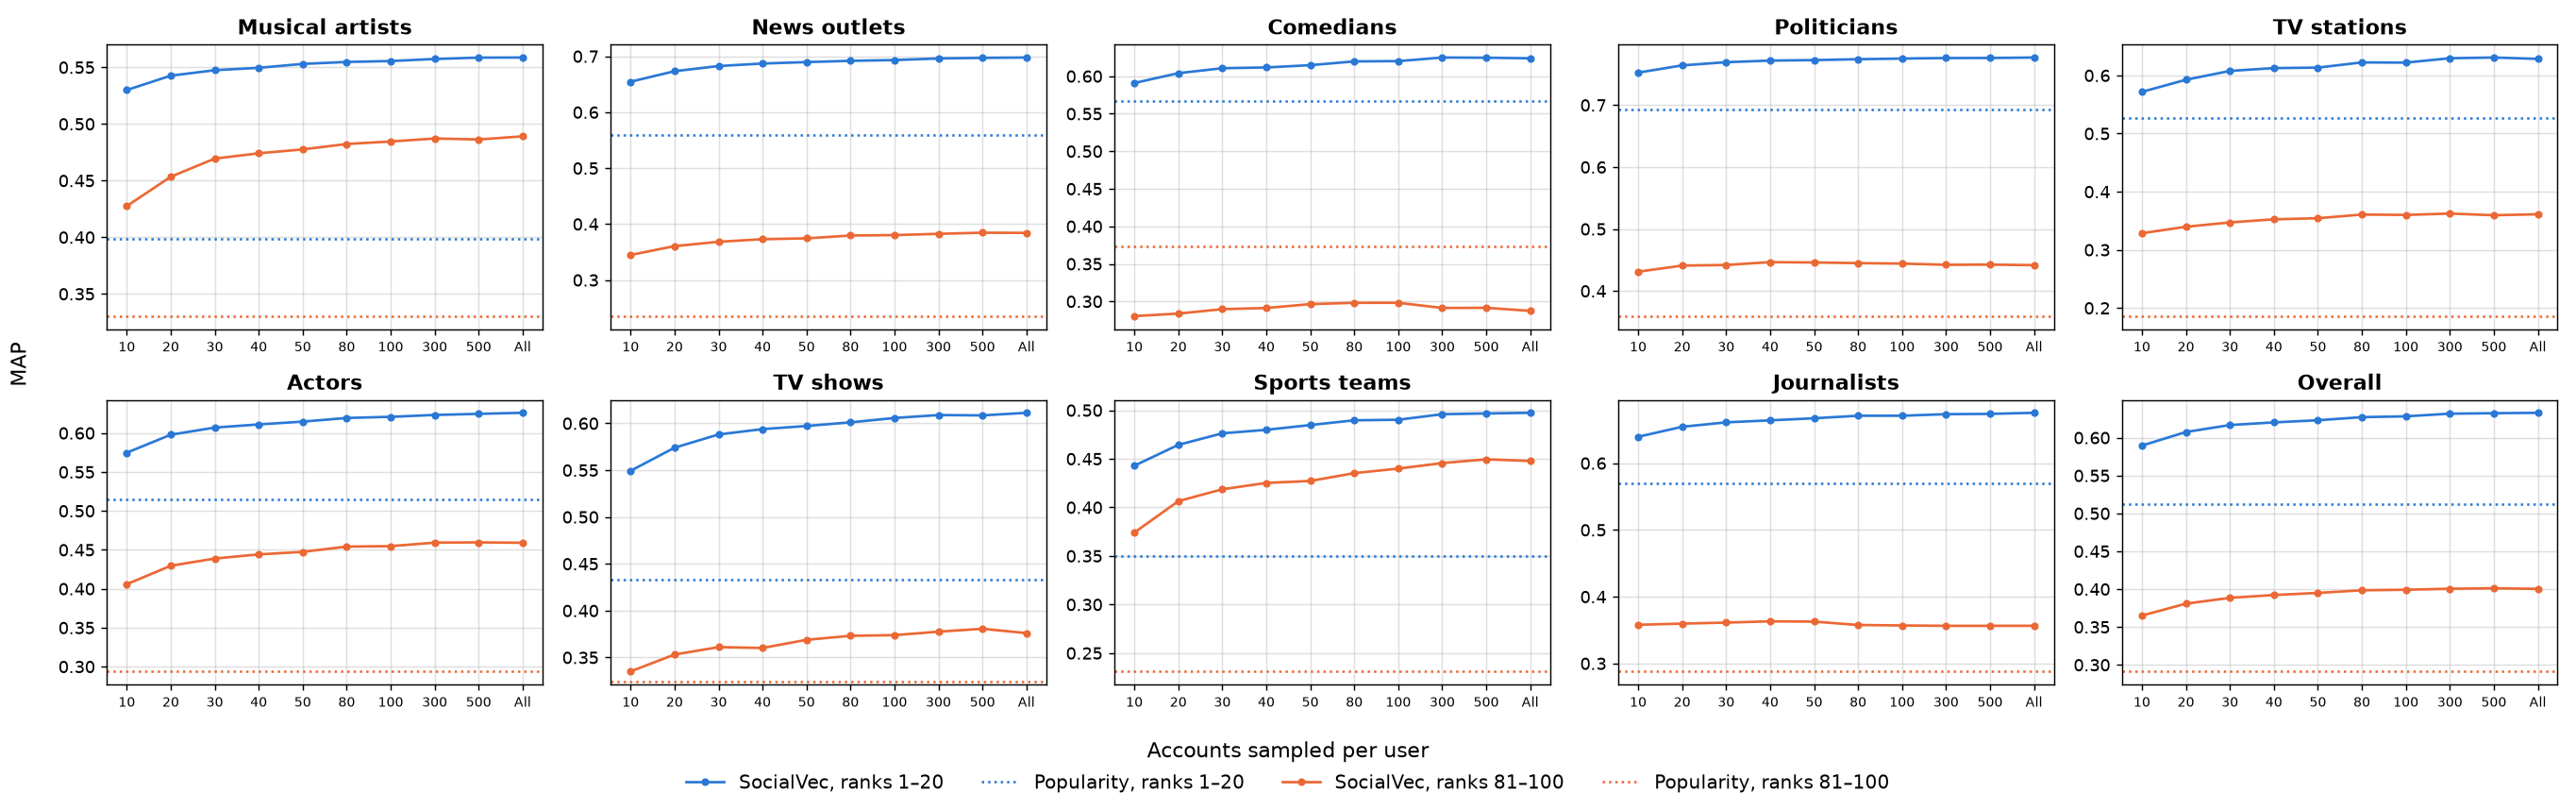
\includegraphics[width=\linewidth]{figures/image_01.png}
\end{center}

\subsection*{How the LLM prompts are built}
The personalized prompts use the authors' wording and list the \textbf{names} of accounts the user follows. The names are the accounts' Twitter display names, as recorded in the SocialVec account metadata (not their handles); accounts without a recorded name are dropped from the list, so a prompt can list fewer accounts than its k. The accounts are drawn at random with a fixed seed (the same draw for a user wherever the condition appears) and listed in the order drawn, which is random:

\begin{itemize}
  \item The target category's own entities are never in this set.
  \item \textbf{k = 50}: drawn from everything the user follows.
\end{itemize}
The candidates to rank are given as a JSON list of ids and names. Where they appear in random order is summarized in Table 14 (Section 4).

\subsection*{Table 3 \textperiodcentered{} LLM personalization per category}
I re-ran the LLM experiment with GPT-6 Luna (reasoning effort \emph{low}) and the authors' prompts, on a stratified random sample of 50 users per category. Listing 12 favored entities lifts MAP from 0.452 to 0.542 (+20\%), and 50 accounts lift it to 0.603 (+33\%). On the same 700 users, SocialVec scores 0.507 with the 12 accounts and 0.511 with the 25 accounts listed in the LLM prompts (k = 50: 0.559), so the LLM is ahead at 12 and 25 accounts, as it is at ranks 81--100 (Table 9).

\begin{center}
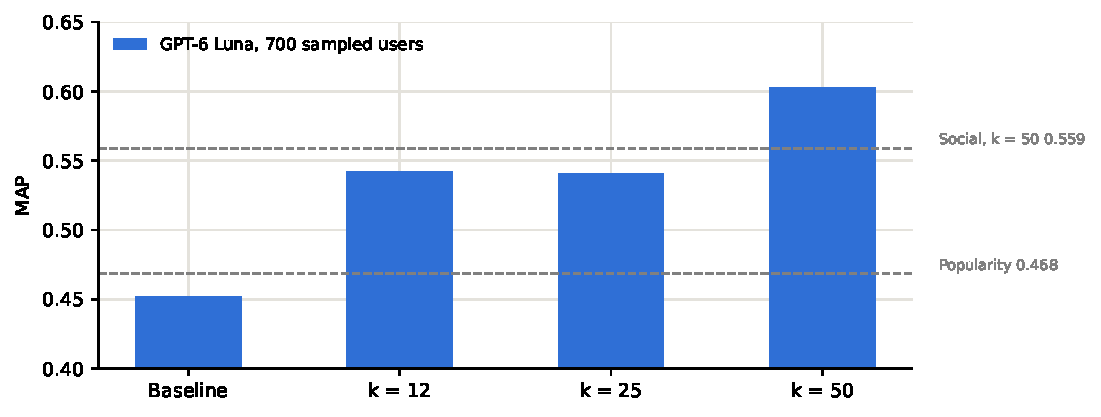
\includegraphics[width=\linewidth,height=0.5\textheight,keepaspectratio]{figures/llm_overall.pdf}
\end{center}

\subsubsection*{Show Table 3 (per category)}
\begin{center}\begin{adjustbox}{max width=\linewidth}
\begin{tabular}{lrrrrrrrr}
\toprule
 & \multicolumn{4}{c}{Same 700 users} & \multicolumn{4}{c}{GPT-6 Luna (700 users)} \\
Category & Popularity & Social, k = 12 & Social, k = 25 & Social, k = 50 & Baseline & k = 12 & k = 25 & k = 50 \\
\midrule
Musical artists & 0.505 & 0.589 & 0.598 & 0.639 & 0.522 & 0.556 & 0.550 & 0.656 \\
News outlets & 0.645 & 0.689 & 0.688 & 0.710 & 0.667 & 0.722 & 0.735 & 0.721 \\
Comedians & 0.545 & 0.563 & 0.563 & 0.600 & 0.541 & 0.628 & 0.640 & 0.642 \\
Politicians & 0.737 & 0.767 & 0.773 & 0.736 & 0.755 & 0.831 & 0.830 & 0.803 \\
TV stations & 0.450 & 0.562 & 0.589 & 0.615 & 0.451 & 0.613 & 0.594 & 0.628 \\
Actors & 0.550 & 0.608 & 0.614 & 0.619 & 0.484 & 0.607 & 0.612 & 0.680 \\
TV shows & 0.364 & 0.576 & 0.567 & 0.603 & 0.405 & 0.604 & 0.575 & 0.649 \\
Sports teams & 0.348 & 0.362 & 0.389 & 0.478 & 0.325 & 0.354 & 0.353 & 0.521 \\
Fashion & 0.332 & 0.356 & 0.352 & 0.435 & 0.321 & 0.402 & 0.416 & 0.533 \\
Journalists & 0.628 & 0.607 & 0.615 & 0.656 & 0.605 & 0.673 & 0.706 & 0.678 \\
TV hosts & 0.336 & 0.355 & 0.369 & 0.412 & 0.274 & 0.424 & 0.425 & 0.485 \\
Films & 0.245 & 0.237 & 0.228 & 0.413 & 0.173 & 0.284 & 0.264 & 0.428 \\
Food chains & 0.441 & 0.442 & 0.439 & 0.498 & 0.418 & 0.429 & 0.436 & 0.496 \\
Car makers & 0.432 & 0.385 & 0.368 & 0.409 & 0.392 & 0.465 & 0.440 & 0.519 \\
\midrule
Overall & 0.468 & 0.507 & 0.511 & 0.559 & 0.452 & 0.542 & 0.541 & 0.603 \\
$\Delta$ vs. LLM baseline &  &  &  &  &  & +20\% & +20\% & +33\% \\
\bottomrule
\end{tabular}

\end{adjustbox}\end{center}

{\small Overall MAP (mean over 14 categories). The dashed reference lines are computed on the same 700 users. The baseline (no user information) is the mean of 10 calls per category with the candidates in random order (Section 4); the personalized prompts list the candidates in one random order per user and condition (Table 14). With the candidates sorted by follower count the baseline scores 0.475. 49\% of the personalized responses had an end-of-output marker appended after the id list, which the original parser scores as a failure. I read the id list itself. Details are in \texttt{results/LLM\_REPORT.md}.}

\subsection*{Table 4 \textperiodcentered{} Categories $\times$ entities per category}
The code behind this table is not in the original notebooks.

\subsubsection*{n per category}
\begin{center}\begin{adjustbox}{max width=\linewidth}
\begin{tabular}{lrrrrrrr}
\toprule
k \textbackslash{} n & 1 & 2 & 3 & 4 & 5 & 6 & 7 \\
\midrule
1 & \cellcolor[HTML]{b7d3f6}\textcolor[HTML]{0b0b0b}{0.472} & \cellcolor[HTML]{9ec5f4}\textcolor[HTML]{0b0b0b}{0.480} & \cellcolor[HTML]{86b6ef}\textcolor[HTML]{0b0b0b}{0.483} & \cellcolor[HTML]{86b6ef}\textcolor[HTML]{0b0b0b}{0.484} & \cellcolor[HTML]{6da7ec}\textcolor[HTML]{0b0b0b}{0.485} & \cellcolor[HTML]{6da7ec}\textcolor[HTML]{0b0b0b}{0.485} & \cellcolor[HTML]{6da7ec}\textcolor[HTML]{0b0b0b}{0.486} \\
2 & \cellcolor[HTML]{6da7ec}\textcolor[HTML]{0b0b0b}{0.489} & \cellcolor[HTML]{3987e5}\textcolor[HTML]{0b0b0b}{0.499} & \cellcolor[HTML]{2a78d6}\textcolor[HTML]{ffffff}{0.501} & \cellcolor[HTML]{2a78d6}\textcolor[HTML]{ffffff}{0.502} & \cellcolor[HTML]{2a78d6}\textcolor[HTML]{ffffff}{0.502} & \cellcolor[HTML]{2a78d6}\textcolor[HTML]{ffffff}{0.502} & \cellcolor[HTML]{2a78d6}\textcolor[HTML]{ffffff}{0.502} \\
3 & \cellcolor[HTML]{2a78d6}\textcolor[HTML]{ffffff}{0.501} & \cellcolor[HTML]{256abf}\textcolor[HTML]{ffffff}{0.507} & \cellcolor[HTML]{256abf}\textcolor[HTML]{ffffff}{0.509} & \cellcolor[HTML]{256abf}\textcolor[HTML]{ffffff}{0.510} & \cellcolor[HTML]{1c5cab}\textcolor[HTML]{ffffff}{0.511} & \cellcolor[HTML]{1c5cab}\textcolor[HTML]{ffffff}{0.511} & \cellcolor[HTML]{1c5cab}\textcolor[HTML]{ffffff}{0.511} \\
4 & \cellcolor[HTML]{256abf}\textcolor[HTML]{ffffff}{0.507} & \cellcolor[HTML]{1c5cab}\textcolor[HTML]{ffffff}{0.513} & \cellcolor[HTML]{1c5cab}\textcolor[HTML]{ffffff}{0.515} & \cellcolor[HTML]{184f95}\textcolor[HTML]{ffffff}{0.516} & \cellcolor[HTML]{184f95}\textcolor[HTML]{ffffff}{0.517} & \cellcolor[HTML]{184f95}\textcolor[HTML]{ffffff}{0.516} & \cellcolor[HTML]{184f95}\textcolor[HTML]{ffffff}{0.517} \\
5 & \cellcolor[HTML]{1c5cab}\textcolor[HTML]{ffffff}{0.511} & \cellcolor[HTML]{184f95}\textcolor[HTML]{ffffff}{0.516} & \cellcolor[HTML]{184f95}\textcolor[HTML]{ffffff}{0.517} & \cellcolor[HTML]{184f95}\textcolor[HTML]{ffffff}{0.518} & \cellcolor[HTML]{184f95}\textcolor[HTML]{ffffff}{0.518} & \cellcolor[HTML]{184f95}\textcolor[HTML]{ffffff}{0.518} & \cellcolor[HTML]{184f95}\textcolor[HTML]{ffffff}{0.519} \\
\bottomrule
\end{tabular}

\end{adjustbox}\end{center}

\subsubsection*{n in total, pooled}
\begin{center}\begin{adjustbox}{max width=\linewidth}
\begin{tabular}{lrrrrrrr}
\toprule
k \textbackslash{} n & 1 & 2 & 3 & 4 & 5 & 6 & 7 \\
\midrule
1 & \cellcolor[HTML]{b7d3f6}\textcolor[HTML]{0b0b0b}{0.473} & \cellcolor[HTML]{86b6ef}\textcolor[HTML]{0b0b0b}{0.481} & \cellcolor[HTML]{86b6ef}\textcolor[HTML]{0b0b0b}{0.484} & \cellcolor[HTML]{6da7ec}\textcolor[HTML]{0b0b0b}{0.485} & \cellcolor[HTML]{6da7ec}\textcolor[HTML]{0b0b0b}{0.485} & \cellcolor[HTML]{6da7ec}\textcolor[HTML]{0b0b0b}{0.486} & \cellcolor[HTML]{6da7ec}\textcolor[HTML]{0b0b0b}{0.486} \\
2 & \cellcolor[HTML]{9ec5f4}\textcolor[HTML]{0b0b0b}{0.476} & \cellcolor[HTML]{6da7ec}\textcolor[HTML]{0b0b0b}{0.489} & \cellcolor[HTML]{5598e7}\textcolor[HTML]{0b0b0b}{0.495} & \cellcolor[HTML]{3987e5}\textcolor[HTML]{0b0b0b}{0.498} & \cellcolor[HTML]{3987e5}\textcolor[HTML]{0b0b0b}{0.500} & \cellcolor[HTML]{2a78d6}\textcolor[HTML]{ffffff}{0.501} & \cellcolor[HTML]{2a78d6}\textcolor[HTML]{ffffff}{0.502} \\
3 & \cellcolor[HTML]{9ec5f4}\textcolor[HTML]{0b0b0b}{0.476} & \cellcolor[HTML]{5598e7}\textcolor[HTML]{0b0b0b}{0.491} & \cellcolor[HTML]{2a78d6}\textcolor[HTML]{ffffff}{0.500} & \cellcolor[HTML]{2a78d6}\textcolor[HTML]{ffffff}{0.504} & \cellcolor[HTML]{256abf}\textcolor[HTML]{ffffff}{0.506} & \cellcolor[HTML]{256abf}\textcolor[HTML]{ffffff}{0.509} & \cellcolor[HTML]{256abf}\textcolor[HTML]{ffffff}{0.509} \\
4 & \cellcolor[HTML]{9ec5f4}\textcolor[HTML]{0b0b0b}{0.478} & \cellcolor[HTML]{5598e7}\textcolor[HTML]{0b0b0b}{0.493} & \cellcolor[HTML]{3987e5}\textcolor[HTML]{0b0b0b}{0.499} & \cellcolor[HTML]{2a78d6}\textcolor[HTML]{ffffff}{0.504} & \cellcolor[HTML]{256abf}\textcolor[HTML]{ffffff}{0.507} & \cellcolor[HTML]{1c5cab}\textcolor[HTML]{ffffff}{0.510} & \cellcolor[HTML]{1c5cab}\textcolor[HTML]{ffffff}{0.513} \\
5 & \cellcolor[HTML]{9ec5f4}\textcolor[HTML]{0b0b0b}{0.478} & \cellcolor[HTML]{5598e7}\textcolor[HTML]{0b0b0b}{0.495} & \cellcolor[HTML]{2a78d6}\textcolor[HTML]{ffffff}{0.502} & \cellcolor[HTML]{256abf}\textcolor[HTML]{ffffff}{0.505} & \cellcolor[HTML]{256abf}\textcolor[HTML]{ffffff}{0.508} & \cellcolor[HTML]{1c5cab}\textcolor[HTML]{ffffff}{0.511} & \cellcolor[HTML]{1c5cab}\textcolor[HTML]{ffffff}{0.514} \\
\bottomrule
\end{tabular}

\end{adjustbox}\end{center}

{\small Overall MAP. Rows: k categories; columns: n entities. Darker cells mean higher MAP (scale 0.465--0.525).}

\subsection*{Figure 2 \textperiodcentered{} Socio-demographic profiles of followers}
User embeddings are classified with SocialVec's five trait classifiers, which I ported to NumPy.

\begin{center}
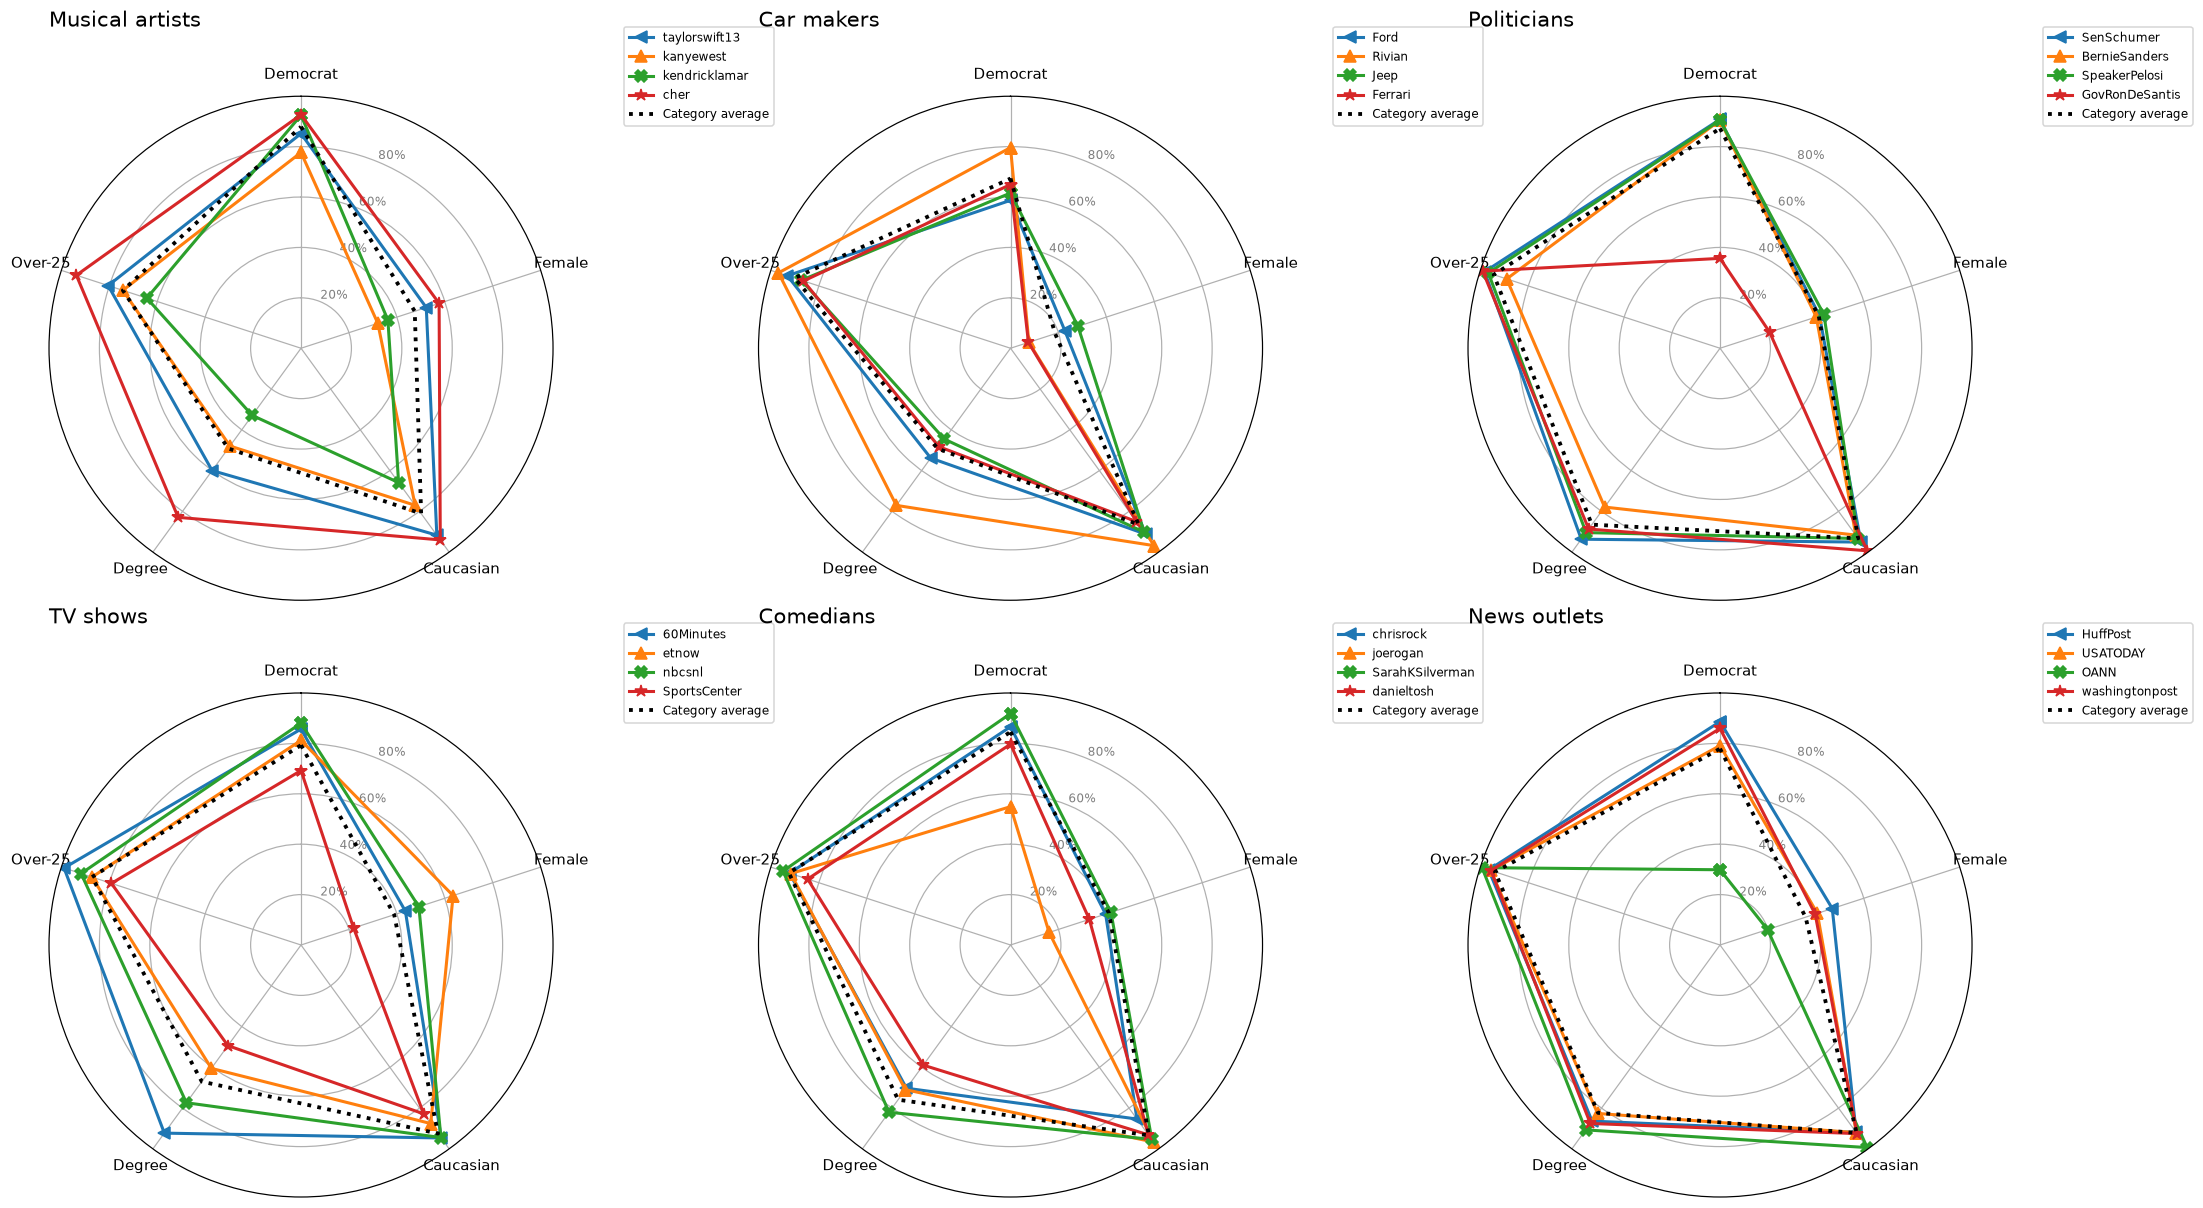
\includegraphics[width=\linewidth]{figures/image_02.png}
\end{center}

\section{Notes on the original code}
Things I found while matching the notebooks.

\noindent\textsc{bug}\par
\subsubsection*{Target entities were never removed}
The "All" profile subtracts screen names from a set of numeric ids, which removes nothing, so the target category stays in the profile. Removing it properly moves overall MAP from 0.621 to 0.617 (+24\% $\rightarrow$ +24\%).

\noindent\textsc{sampling}\par
\subsubsection*{SE1 samples can't be redrawn exactly}
The original order came from a set of string ids, which changes with every Python run. Redrawn with the same seed, the overall values land within $\pm$0.004. The closed-world (SE2) samples match exactly.

\noindent\textsc{detail}\par
\subsubsection*{"Entities" are followed accounts}
SE1 samples k followed \emph{accounts}, and only about 43\% of them are SocialVec entities.

\section{Extension \textperiodcentered{} Less popular entities}
Does social user modeling still help when the candidates aren't the most famous entities in their category?

In the 9 categories that list 100 typed entities, I sorted the entities by Twitter follower count and ranked those at positions \textbf{81--100} instead of the top 20. No original sheet lists more. User profiles exclude \emph{every} entity known to belong to the target category: its original sheet, its top-20 list and its extended list, so none of the 40 candidates (ranks 1--20 and 81--100) is in any profile. The main setup (Table 6) evaluates each of the 11,153 users in every category in which they follow at least one entity of the band; as a matched control, the original top 20 are ranked for the same users with the same profiles. Table 5 repeats this for only the users sampled for each category. A random ranking (exact expected AP) provides a chance level, and paired Wilcoxon tests compare the two methods.

\begin{itemize}
  \item \textbf{Popularity breaks down in the tail.} On all 36,739 user--category pairs, at ranks 81--100 it scores 0.291, barely above a random ranking (0.252), and below it for News outlets, Politicians, TV stations and Journalists.
  \item \textbf{Social similarity holds up.} It scores 0.400, above chance in 9 of 9 categories, and beats popularity in 8 of 9. Its relative gain over popularity grows from +23\% on the top 20 to +37\% (p \textless{} 0.001 overall and in every category).
  \item \textbf{The matched control on the users sampled for each category agrees.} On those 3,798 users the gain is +22\% on the top 20 and +38\% at ranks 81--100 (Table 5).
  \item \textbf{The exception is Comedians ($-$23\%).} Follows in that band concentrate on its two most-followed accounts, both mainly political commentators, which popularity ranks first.
\end{itemize}
\subsubsection*{Original top 20}
{\small Same user--category pairs and profiles as on the right}

\begin{center}
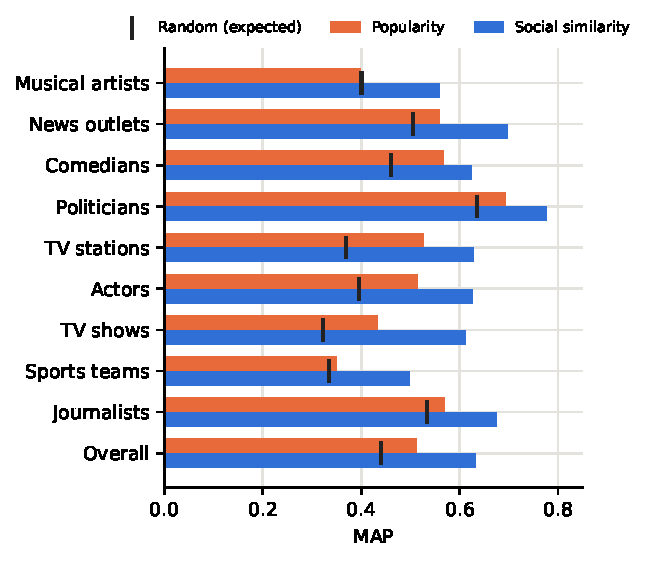
\includegraphics[width=\linewidth,height=0.5\textheight,keepaspectratio]{figures/section3_ranks_1_20.pdf}
\end{center}

\subsubsection*{Ranks 81--100}
{\small All experiment users who follow a band entity}

\begin{center}
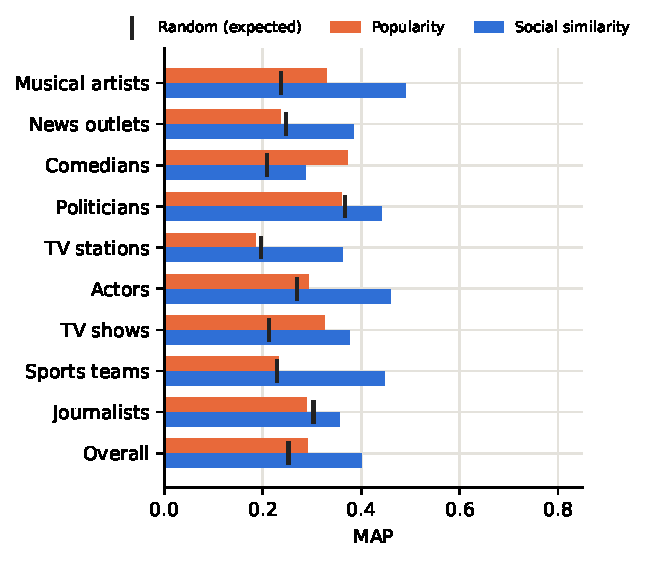
\includegraphics[width=\linewidth,height=0.5\textheight,keepaspectratio]{figures/section3_ranks_81_100.pdf}
\end{center}

{\small MAP per category; $\Delta$ is the gain of social similarity over popularity. The values are in Table 6 below.}

\subsection*{Table 5 \textperiodcentered{} Ranks 81--100 vs. top 20, users sampled for each category}
\begin{center}\begin{adjustbox}{max width=\linewidth}
\begin{tabular}{lrrrrrrrrrrrrr}
\toprule
 &  & \multicolumn{6}{c}{Ranks 1--20 (original candidates)} & \multicolumn{6}{c}{Ranks 81--100} \\
Category & Users & Rel./user & Random & Popularity & Social & $\Delta$ & p & Rel./user & Random & Popularity & Social & $\Delta$ & p \\
\midrule
Musical artists & 472 & 8.1 & 0.488 & 0.518 & 0.651 & +26\% & \textless{} 0.001 & 2.4 & 0.240 & 0.349 & 0.519 & +49\% & \textless{} 0.001 \\
News outlets & 426 & 9.4 & 0.542 & 0.604 & 0.731 & +21\% & \textless{} 0.001 & 2.5 & 0.244 & 0.233 & 0.376 & +61\% & \textless{} 0.001 \\
Comedians & 277 & 9.0 & 0.526 & 0.617 & 0.678 & +10\% & \textless{} 0.001 & 1.8 & 0.214 & 0.363 & 0.266 & $-$27\% & \textless{} 0.001 \\
Politicians & 641 & 12.3 & 0.695 & 0.734 & 0.802 & +9\% & \textless{} 0.001 & 5.6 & 0.377 & 0.359 & 0.431 & +20\% & \textless{} 0.001 \\
TV stations & 198 & 6.4 & 0.412 & 0.527 & 0.671 & +27\% & \textless{} 0.001 & 1.4 & 0.198 & 0.186 & 0.412 & +121\% & \textless{} 0.001 \\
Actors & 579 & 7.4 & 0.456 & 0.560 & 0.693 & +24\% & \textless{} 0.001 & 3.2 & 0.274 & 0.305 & 0.476 & +56\% & \textless{} 0.001 \\
TV shows & 216 & 5.4 & 0.371 & 0.429 & 0.674 & +57\% & \textless{} 0.001 & 1.4 & 0.215 & 0.325 & 0.397 & +22\% & 0.014 \\
Sports teams & 240 & 6.9 & 0.437 & 0.441 & 0.575 & +31\% & \textless{} 0.001 & 2.5 & 0.245 & 0.260 & 0.431 & +66\% & \textless{} 0.001 \\
Journalists & 749 & 11.4 & 0.628 & 0.666 & 0.719 & +8\% & \textless{} 0.001 & 4.1 & 0.325 & 0.299 & 0.381 & +28\% & \textless{} 0.001 \\
\midrule
Overall & 3,798 &  & 0.506 & 0.566 & 0.688 & +22\% & \textless{} 0.001 &  & 0.259 & 0.298 & 0.410 & +38\% & \textless{} 0.001 \\
\bottomrule
\end{tabular}

\end{adjustbox}\end{center}

{\small 3,798 users who follow at least one entity ranked 81--100 in their category. Rel./user is the number of candidates a user follows. Dotted red marks popularity scores below the random ranking. p is from a Wilcoxon signed-rank test, social vs. popularity.}

\subsection*{Table 6 \textperiodcentered{} Ranks 81--100 vs. top 20, all experiment users}
The main setup. Each of the 11,153 users is evaluated in every category in which they follow at least one entity from each band. That gives 36,739 user--category pairs from 10,039 distinct users; only 10\% of these pairs come from users sampled for the category (Table 5). The overall test pools all pairs. The candidates are listed in Table 7.

\begin{center}\begin{adjustbox}{max width=\linewidth}
\begin{tabular}{lrrrrrrrrrrrrr}
\toprule
 &  & \multicolumn{6}{c}{Ranks 1--20 (original candidates)} & \multicolumn{6}{c}{Ranks 81--100} \\
Category & Users & Rel./user & Random & Popularity & Social & $\Delta$ & p & Rel./user & Random & Popularity & Social & $\Delta$ & p \\
\midrule
Musical artists & 5,922 & 6.1 & 0.401 & 0.398 & 0.559 & +40\% & \textless{} 0.001 & 2.3 & 0.238 & 0.330 & 0.489 & +48\% & \textless{} 0.001 \\
News outlets & 4,426 & 8.5 & 0.505 & 0.560 & 0.698 & +25\% & \textless{} 0.001 & 2.6 & 0.248 & 0.235 & 0.384 & +63\% & \textless{} 0.001 \\
Comedians & 2,528 & 7.5 & 0.460 & 0.567 & 0.624 & +10\% & \textless{} 0.001 & 1.7 & 0.209 & 0.373 & 0.287 & $-$23\% & \textless{} 0.001 \\
Politicians & 6,348 & 10.9 & 0.636 & 0.693 & 0.777 & +12\% & \textless{} 0.001 & 5.3 & 0.366 & 0.359 & 0.442 & +23\% & \textless{} 0.001 \\
TV stations & 2,585 & 5.4 & 0.369 & 0.527 & 0.628 & +19\% & \textless{} 0.001 & 1.4 & 0.197 & 0.186 & 0.361 & +94\% & \textless{} 0.001 \\
Actors & 6,064 & 6.0 & 0.395 & 0.515 & 0.626 & +22\% & \textless{} 0.001 & 3.1 & 0.270 & 0.294 & 0.459 & +56\% & \textless{} 0.001 \\
TV shows & 2,769 & 4.3 & 0.323 & 0.433 & 0.611 & +41\% & \textless{} 0.001 & 1.4 & 0.213 & 0.325 & 0.376 & +16\% & \textless{} 0.001 \\
Sports teams & 1,585 & 4.6 & 0.334 & 0.350 & 0.497 & +42\% & \textless{} 0.001 & 2.1 & 0.229 & 0.231 & 0.448 & +94\% & \textless{} 0.001 \\
Journalists & 4,512 & 9.2 & 0.534 & 0.570 & 0.675 & +19\% & \textless{} 0.001 & 3.6 & 0.303 & 0.288 & 0.356 & +24\% & \textless{} 0.001 \\
\midrule
Overall & 36,739 &  & 0.440 & 0.513 & 0.633 & +23\% & \textless{} 0.001 &  & 0.252 & 0.291 & 0.400 & +37\% & \textless{} 0.001 \\
\bottomrule
\end{tabular}

\end{adjustbox}\end{center}

\subsubsection*{Table 7 \textperiodcentered{} Candidate entities, ranks 81--100 (entity name with its Twitter handle; * no SocialVec embedding, excluded)}
\begin{center}\begin{adjustbox}{max width=\linewidth}
\begin{tabular}{lrp{0.75\linewidth}}
\toprule
Category & Followers & Entities \\
\midrule
Musical artists & 23K -- 1,482K & Ice-T {\textcolor{gray}{(@FINALLEVEL)}}, Teyana Taylor {\textcolor{gray}{(@TEYANATAYLOR)}}, Janelle Monáe {\textcolor{gray}{(@JanelleMonae)}}, Bruce Springsteen {\textcolor{gray}{(@springsteen)}}, Doja Cat {\textcolor{gray}{(@DojaCat)}}, Summer Walker {\textcolor{gray}{(@IAMSUMMERWALKER)}}, Moneybagg Yo {\textcolor{gray}{(@MoneyBaggYo)}}, Kid Rock {\textcolor{gray}{(@KidRock)}}, Barbra Streisand {\textcolor{gray}{(@BarbraStreisand)}}, Tom Morello {\textcolor{gray}{(@tmorello)}}, Polo G {\textcolor{gray}{(@Polo\_Capalot)}}, Ari Lennox {\textcolor{gray}{(@AriLennox)}}, Ted Nugent {\textcolor{gray}{(@TedNugent)}}, Kaya Jones {\textcolor{gray}{(@KayaJones)}}, Scott Gottlieb, MD {\textcolor{gray}{(@ScottGottliebMD)}}, Richard Marx {\textcolor{gray}{(@richardmarx)}}, Nancy Sinatra {\textcolor{gray}{(@NancySinatra)}}, John Rich {\textcolor{gray}{(@johnrich)}}, Travis Tritt {\textcolor{gray}{(@Travistritt)}}, Dionne Warwick {\textcolor{gray}{(@\_DionneWarwick)}} \\
News outlets & 74K -- 325K & Harris Faulkner {\textcolor{gray}{(@HARRISFAULKNER)}}, All Things Considered {\textcolor{gray}{(@npratc)}}, Erin Burnett {\textcolor{gray}{(@ErinBurnett)}}, Twitchy Team {\textcolor{gray}{(@TwitchyTeam)}}, BNO Newsroom {\textcolor{gray}{(@BNODesk)}}, BlazeTV {\textcolor{gray}{(@BlazeTV)}}, Washington Examiner {\textcolor{gray}{(@dcexaminer)}}, Texas Tribune {\textcolor{gray}{(@TexasTribune)}}, Heather Childers {\textcolor{gray}{(@HeatherChilders)}}, RealClearPolitics {\textcolor{gray}{(@RealClearNews)}}, Mediaite {\textcolor{gray}{(@Mediaite)}}, Townhall.com {\textcolor{gray}{(@townhallcom)}}, Dagen McDowell {\textcolor{gray}{(@dagenmcdowell)}}, Karen Attiah {\textcolor{gray}{(@KarenAttiah)}}, BNO News {\textcolor{gray}{(@BNONews)}}, Goldie Taylor {\textcolor{gray}{(@goldietaylor)}}, Bianna Golodryga {\textcolor{gray}{(@biannagolodryga)}}, John Berman {\textcolor{gray}{(@JohnBerman)}}, Newsmax {\textcolor{gray}{(@newsmax)}}, Ana Cabrera {\textcolor{gray}{(@AnaCabrera)}} \\
Comedians & 22K -- 106K & Dean Obeidallah {\textcolor{gray}{(@DeanObeidallah)}}, Hal Sparks {\textcolor{gray}{(@HalSparks)}}, Nate Bargatze {\textcolor{gray}{(@natebargatze)}}, Melissa Villaseñor {\textcolor{gray}{(@melissavcomedy)}}, Sara Schaefer {\textcolor{gray}{(@saraschaefer1)}}, Daniel Kibblesmith {\textcolor{gray}{(@kibblesmith)}}, Gary Gulman {\textcolor{gray}{(@GaryGulman)}}, James Adomian {\textcolor{gray}{(@JAdomian)}}, Phoebe Robinson {\textcolor{gray}{(@dopequeenpheebs)}}, Steve Hofstetter {\textcolor{gray}{(@SteveHofstetter)}}, Lily Tomlin {\textcolor{gray}{(@LilyTomlin)}}, Blaine Capatch {\textcolor{gray}{(@blainecapatch)}}, Laurie Kilmartin {\textcolor{gray}{(@anylaurie16)}}, Tom Shillue {\textcolor{gray}{(@tomshillue)}}, Aamer Rahman {\textcolor{gray}{(@aamer\_rahman)}}, Sam Morril {\textcolor{gray}{(@sammorril)}}, Jena Friedman {\textcolor{gray}{(@JenaFriedman)}}, Karen Chee {\textcolor{gray}{(@karencheee)}}, Jackie Kashian {\textcolor{gray}{(@jackiekashian)}}, Yannis Pappas {\textcolor{gray}{(@yannispappas)}} \\
Politicians & 20K -- 328K & Mark Kelly {\textcolor{gray}{(@CaptMarkKelly)}}, Brian Schatz {\textcolor{gray}{(@brianschatz)}}, Jaime Harrison {\textcolor{gray}{(@harrisonjaime)}}, Rep. Pramila Jayapal {\textcolor{gray}{(@RepJayapal)}}, John Dean {\textcolor{gray}{(@JohnWDean)}}, Hakeem Jeffries {\textcolor{gray}{(@RepJeffries)}}, Karine Jean-Pierre {\textcolor{gray}{(@K\_JeanPierre)}}, Sherrilyn Ifill {\textcolor{gray}{(@Sifill\_LDF)}}, Josh Hawley {\textcolor{gray}{(@HawleyMO)}}, Sen. Marsha Blackburn {\textcolor{gray}{(@MarshaBlackburn)}}, Ronald Klain {\textcolor{gray}{(@RonaldKlain)}}, Thomas Massie {\textcolor{gray}{(@RepThomasMassie)}}, Jon Ossoff {\textcolor{gray}{(@ossoff)}}, Rep. Jamie Raskin {\textcolor{gray}{(@RepRaskin)}}, Raja Krishnamoorthi {\textcolor{gray}{(@CongressmanRaja)}}, John Fetterman {\textcolor{gray}{(@JohnFetterman)}}, Jen Psaki {\textcolor{gray}{(@jrpsaki)}}, Cori Bush {\textcolor{gray}{(@CoriBush)}}, Josh Shapiro {\textcolor{gray}{(@JoshShapiroPA)}}, Nikki Fried {\textcolor{gray}{(@nikkifried)}} \\
TV stations & 18K -- 214K & 12 News {\textcolor{gray}{(@12News)}}, WESH 2 News {\textcolor{gray}{(@WESH)}}, Logo {\textcolor{gray}{(@LogoTV)}}, STARZ {\textcolor{gray}{(@STARZ)}}, TCM {\textcolor{gray}{(@tcm)}}, KXAN News {\textcolor{gray}{(@KXAN\_News)}}, WeatherNation {\textcolor{gray}{(@WeatherNation)}}, Hawaii News Now {\textcolor{gray}{(@HawaiiNewsNow)}}, ABC 7 News - WJLA {\textcolor{gray}{(@ABC7News)}}, HBO Documentaries {\textcolor{gray}{(@HBODocs)}}, CNN Communications {\textcolor{gray}{(@CNNPR)}}, SNY {\textcolor{gray}{(@SNYtv)}}, SportsNet LA {\textcolor{gray}{(@SportsNetLA)}}, Celtics on NBC Sports Boston {\textcolor{gray}{(@NBCSCeltics)}}, Florida Democrats {\textcolor{gray}{(@FlaDems)}}, MSG Networks {\textcolor{gray}{(@MSGNetworks)}}, NBCSports Washington {\textcolor{gray}{(@NBCSWashington)}}, SYFY WIRE {\textcolor{gray}{(@SYFYWIRE)}}, NC Democratic Party {\textcolor{gray}{(@NCDemParty)}}, New York GOP {\textcolor{gray}{(@NewYorkGOP)}} \\
Actors & 101K -- 464K & Michael Rapaport {\textcolor{gray}{(@MichaelRapaport)}}, Pedro Pascal {\textcolor{gray}{(@PedroPascal1)}}, Yvette Nicole Brown {\textcolor{gray}{(@YNB)}}, Patricia Arquette {\textcolor{gray}{(@PattyArquette)}}, Dean Cain {\textcolor{gray}{(@RealDeanCain)}}, Tara Strong {\textcolor{gray}{(@tarastrong)}}, Sacha Baron Cohen {\textcolor{gray}{(@SachaBaronCohen)}}, Carl Reiner {\textcolor{gray}{(@carlreiner)}}, Chris Meloni {\textcolor{gray}{(@Chris\_Meloni)}}, Adam Baldwin {\textcolor{gray}{(@AdamBaldwin)}}, Bradley Whitford {\textcolor{gray}{(@BradleyWhitford)}}, Jon Voight {\textcolor{gray}{(@jonvoight)}}, Halle Berry {\textcolor{gray}{(@halleberry)}}, Tom Arnold {\textcolor{gray}{(@TomArnold)}}, Kristy Swanson {\textcolor{gray}{(@KristySwansonXO)}}, Ellen Barkin {\textcolor{gray}{(@EllenBarkin)}}, Ken Olin {\textcolor{gray}{(@kenolin1)}}, Kristen Johnston {\textcolor{gray}{(@thekjohnston)}}, Rosanna Arquette {\textcolor{gray}{(@RoArquette)}}, Morgan Fairchild {\textcolor{gray}{(@morgfair)}} \\
TV shows & 46K -- 254K & Jeopardy! {\textcolor{gray}{(@Jeopardy)}}, CBS Sunday Morning {\textcolor{gray}{(@CBSSunday)}}, Dragon Age {\textcolor{gray}{(@dragonage)}}, Trailer Park Boys {\textcolor{gray}{(@trailerparkboys)}}, Bravo Top Chef All Stars LA {\textcolor{gray}{(@BravoTopChef)}}, Squawk Box {\textcolor{gray}{(@SquawkCNBC)}}, Ancient Aliens {\textcolor{gray}{(@AncientAliens)}}, Seinfeld {\textcolor{gray}{(@SeinfeldTV)}}, Drunk History {\textcolor{gray}{(@drunkhistory)}}, grown-ish {\textcolor{gray}{(@grownish)}}, Queen Sugar {\textcolor{gray}{(@QueenSugarOWN)}}, The Orville {\textcolor{gray}{(@TheOrville)}}, Suda51 (Goichi Suda) {\textcolor{gray}{(@suda\_51)}}, Mystery Science Theater 3000 {\textcolor{gray}{(@MST3K)}}, Washington Journal {\textcolor{gray}{(@cspanwj)}}, Cobra Kai {\textcolor{gray}{(@CobraKaiSeries)}}, The Kelly Clarkson Show {\textcolor{gray}{(@KellyClarksonTV)}}\textsuperscript{*}, RWBY {\textcolor{gray}{(@OfficialRWBY)}}\textsuperscript{*}, 2020 Democratic National Convention {\textcolor{gray}{(@DemConvention)}}, Svengoolie {\textcolor{gray}{(@Svengoolie)}} \\
Sports teams & 221K -- 588K & Team Liquid {\textcolor{gray}{(@TeamLiquid)}}, Tampa Bay Rays {\textcolor{gray}{(@RaysBaseball)}}, Oakland A's {\textcolor{gray}{(@Athletics)}}, Seattle Mariners {\textcolor{gray}{(@Mariners)}}, Evil Geniuses {\textcolor{gray}{(@EvilGeniuses)}}, New York Islanders {\textcolor{gray}{(@NYIslanders)}}, Columbus Blue Jackets {\textcolor{gray}{(@BlueJacketsNHL)}}, Vegas Golden Knights {\textcolor{gray}{(@GoldenKnights)}}, Star Trek {\textcolor{gray}{(@StarTrek)}}, CLG {\textcolor{gray}{(@clgaming)}}, New York City FC {\textcolor{gray}{(@NYCFC)}}, Luminosity Gaming {\textcolor{gray}{(@Luminosity)}}, Florida Panthers {\textcolor{gray}{(@FlaPanthers)}}, Miami Marlins {\textcolor{gray}{(@Marlins)}}, USA Hockey {\textcolor{gray}{(@usahockey)}}, Florida Gators {\textcolor{gray}{(@FloridaGators)}}, UNC Tar Heels {\textcolor{gray}{(@GoHeels)}}, Yankees PR Dept. {\textcolor{gray}{(@YankeesPR)}}, Complexity Gaming {\textcolor{gray}{(@Complexity)}}, TRENT? {\textcolor{gray}{(@trentylocks)}} \\
Journalists & 51K -- 147K & Carl Bernstein {\textcolor{gray}{(@carlbernstein)}}, Peter Doocy {\textcolor{gray}{(@pdoocy)}}, Michael Tracey {\textcolor{gray}{(@mtracey)}}, Susan Glasser {\textcolor{gray}{(@sbg1)}}, Ari Berman {\textcolor{gray}{(@AriBerman)}}, Taylor Lorenz {\textcolor{gray}{(@TaylorLorenz)}}, Jonathan Lemire {\textcolor{gray}{(@JonLemire)}}, Catherine Herridge {\textcolor{gray}{(@CBS\_Herridge)}}\textsuperscript{*}, Elie Mystal {\textcolor{gray}{(@ElieNYC)}}, Jennifer Griffin {\textcolor{gray}{(@JenGriffinFNC)}}, Jason Leopold {\textcolor{gray}{(@JasonLeopold)}}, Carol Leonnig {\textcolor{gray}{(@CarolLeonnig)}}, Adam Housley {\textcolor{gray}{(@adamhousley)}}, Kyle Cheney {\textcolor{gray}{(@kyledcheney)}}, Will Sommer {\textcolor{gray}{(@willsommer)}}, Jeremy Diamond {\textcolor{gray}{(@JDiamond1)}}, Clarissa Ward {\textcolor{gray}{(@clarissaward)}}, Paula Reid {\textcolor{gray}{(@PaulaReidCBS)}}, Andrew Feinberg {\textcolor{gray}{(@AndrewFeinberg)}}, E. Jean Carroll {\textcolor{gray}{(@ejeancarroll)}} \\
\bottomrule
\end{tabular}

\end{adjustbox}\end{center}

\subsection*{How popular are the candidates overall?}
The bands are defined within each category. To see where the candidates stand among all accounts, I placed every candidate in the popularity ranking of all 201,346 SocialVec accounts, which are sorted by how many users follow them (rank 1 is the most followed). In these 9 categories, the original top 20 have a median global rank of 405; the ranks 81--100 candidates 13,672, with 38\% of them in the global top 10,000.

\subsubsection*{Figure 3 \textperiodcentered{} Global popularity of the candidates, by category}
\begin{center}
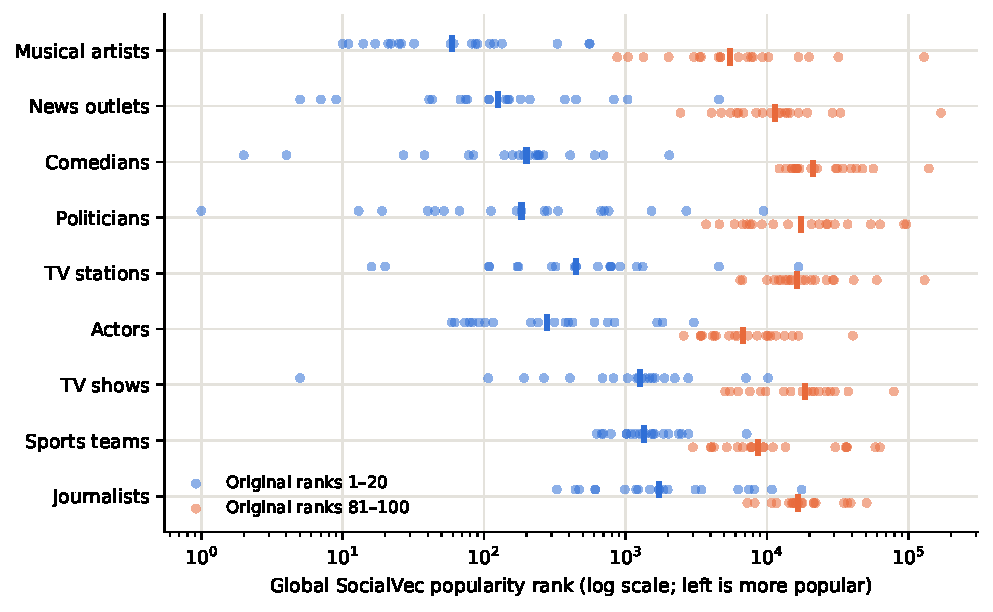
\includegraphics[width=\linewidth,height=0.5\textheight,keepaspectratio]{figures/figure3_global_popularity.pdf}
\end{center}

{\small Global SocialVec popularity rank of every candidate (log scale; left is more popular), by category. Each dot is one account; the bar marks the band's median. 3 candidates without a SocialVec embedding are not shown.}

\subsection*{Table 8 \textperiodcentered{} Global popularity of the candidates}
\begin{center}\begin{adjustbox}{max width=\linewidth}
\begin{tabular}{lrrrrrrrrrr}
\toprule
 & \multicolumn{4}{c}{Global rank at category position} & \multicolumn{2}{c}{Median global rank} & \multicolumn{2}{c}{In the global top 10,000} & \multicolumn{2}{c}{Median followers} \\
Category & 1 & 20 & 81 & 100 & 1--20 & 81--100 & 1--20 & 81--100 & 1--20 & 81--100 \\
\midrule
Musical artists & 22 & 236 & 874 & 129,478 & 60 & 5,502 & 100\% & 75\% & 32,894,506 & 552,766 \\
News outlets & 7 & 74 & 6,308 & 33,230 & 126 & 11,438 & 100\% & 45\% & 12,742,284 & 162,872 \\
Comedians & 2 & 527 & 16,294 & 139,819 & 200 & 21,135 & 100\% & 0\% & 8,229,776 & 82,468 \\
Politicians & 1 & 1,238 & 3,717 & 96,889 & 184 & 17,410 & 100\% & 40\% & 4,446,490 & 158,984 \\
TV stations & 7 & 791 & 17,848 & 130,668 & 448 & 16,393 & 95\% & 10\% & 4,245,468 & 145,691 \\
Actors & 145 & 839 & 2,583 & 15,199 & 278 & 6,776 & 100\% & 65\% & 5,745,956 & 325,924 \\
TV shows & 5 & 1,049 & 5,073 & 28,107 & 1,268 & 18,582 & 95\% & 33\% & 2,201,817 & 102,624 \\
Sports teams & 678 & 1,863 & 36,726 & 30,473 & 1,358 & 8,648 & 100\% & 60\% & 2,248,687 & 398,476 \\
Journalists & 471 & 1,486 & 10,817 & 50,828 & 1,722 & 16,596 & 90\% & 11\% & 682,227 & 114,934 \\
\midrule
Overall &  &  &  &  & 405 & 13,672 & 98\% & 38\% & 3,740,031 & 165,190 \\
\bottomrule
\end{tabular}

\end{adjustbox}\end{center}

{\small Global rank: position among all SocialVec accounts, 1 being the most followed. \emph{Global rank at category position} gives the account at positions 1, 20, 81 and 100 of the category's original sheet sorted by Twitter follower count, the order that defines ranks 81--100 (account name beneath). Overall pools all candidates of the band.}

\subsection*{Table 9 \textperiodcentered{} LLM and SocialVec ranking of ranks 81--100}
The Table 3 protocol applied to the less popular candidates, for 200 random users per category who follow at least one candidate (TV stations have only 198), without 56 organizations and likely bots (below): 1,742 users. Every listed entity of the target category is removed from the prompts. Without user information, the LLM is no better than popularity (0.282 vs. 0.295). With user information it personalizes well: 0.392 with 12 entities and 0.479 with 50 accounts. Social similarity from all of the user's entities scores 0.418. The two are complementary: with 12 entities the LLM is stronger for news outlets, comedians, politicians and journalists; social similarity from all entities for musical artists, TV stations, actors, TV shows and sports teams. Ranking from GPT-4o's demographic description alone (Section 5) scores 0.339, between no user information (0.282) and 12 entities (0.392); it is ahead of 12 entities for musical artists, TV shows and sports teams.

For a like-for-like comparison, the \emph{SocialVec k = 12} and \emph{k = 25} columns build the user embedding from exactly the accounts listed in the LLM's k = 12 and k = 25 prompts (11.7 and 21.7 on average, as some users have fewer). Follow statistics of these 1,742 users: accounts followed: minimum 68, mean 2,232, median 1,934, maximum 5,000; candidate entities followed: minimum 11, mean 48.2, median 44, maximum 147. Given the same evidence, the LLM ranks better at both sizes: 0.392 vs. 0.354 with 12 accounts (paired Wilcoxon p \textless{} 0.001; ahead in 6 of 9 categories), and 0.393 vs. 0.352 with 25 (p \textless{} 0.001; ahead in 7 of 9).

\textbf{Organizations and likely bots.} The profiles of these users (bio, follower, tweet and like counts and account age, as collected) were screened: 21 are organizations (an organization keyword search of bios and handles, every match read by hand) and 3 more possibly are; 11 post more than 144 tweets a day on average over the account's life; and 21 show at least two weaker bot signals (more than 72 tweets a day, following 4,900 or more accounts, followers under 5\% of follows, a handle ending in six or more digits with an empty bio, no likes, an account under 90 days old). No profile looked like a clear bot, so the 56 are a cautious upper bound. They are left out of Table 9--Table 11 and Section 5.

The \emph{k = 6 of 50}, \emph{k = 12 of 50} and \emph{k = 25 of 50} columns draw 6, 12 and 25 names from the user's k = 50 list instead of the closed set; \emph{k = 6} lists the first 6 names of the closed-set k = 12 prompt (see Table 23 in Section 5).

\begin{center}\begin{adjustbox}{max width=\linewidth}
\begin{tabular}{lrrrrrrrrrrrrr}
\toprule
 &  & \multicolumn{2}{c}{Non-personalized} & \multicolumn{3}{c}{SocialVec} & \multicolumn{7}{c}{GPT-6 Luna} \\
Category & Users & Random & Popularity & All entities & k = 12 & k = 25 & Baseline & Demographics & k = 12 & k = 25 & k = 12 of 50 & k = 25 of 50 & k = 50 \\
\midrule
Musical artists & 196 & 0.240 & 0.345 & \textbf{0.528} & 0.421 & 0.423 & 0.257 & 0.381 & 0.336 & 0.330 & 0.435 & 0.441 & 0.471 \\
News outlets & 189 & 0.241 & 0.215 & 0.382 & 0.295 & 0.304 & 0.251 & 0.278 & 0.438 & 0.437 & 0.441 & \textbf{0.460} & 0.447 \\
Comedians & 198 & 0.213 & 0.371 & 0.271 & 0.316 & 0.304 & 0.199 & 0.240 & 0.358 & 0.369 & 0.384 & 0.386 & \textbf{0.394} \\
Politicians & 196 & 0.369 & 0.347 & 0.454 & 0.414 & 0.411 & 0.396 & 0.439 & 0.518 & 0.522 & 0.552 & \textbf{0.569} & 0.552 \\
TV stations & 189 & 0.197 & 0.186 & 0.414 & 0.306 & 0.305 & 0.193 & 0.257 & 0.369 & 0.363 & 0.521 & \textbf{0.558} & 0.524 \\
Actors & 198 & 0.272 & 0.309 & 0.480 & 0.400 & 0.391 & 0.325 & 0.392 & 0.410 & 0.411 & 0.471 & 0.467 & \textbf{0.489} \\
TV shows & 192 & 0.215 & 0.334 & 0.396 & 0.379 & 0.379 & 0.327 & 0.378 & 0.366 & 0.362 & 0.402 & \textbf{0.449} & 0.444 \\
Sports teams & 190 & 0.245 & 0.255 & 0.445 & 0.310 & 0.310 & 0.231 & 0.315 & 0.302 & 0.322 & 0.473 & 0.488 & \textbf{0.519} \\
Journalists & 194 & 0.321 & 0.295 & 0.392 & 0.341 & 0.340 & 0.359 & 0.372 & 0.428 & 0.422 & \textbf{0.475} & 0.475 & 0.473 \\
\midrule
Overall & 1,742 & 0.257 & 0.295 & 0.418 & 0.354 & 0.352 & 0.282 & 0.339 & 0.392 & 0.393 & 0.461 & 0.477 & \textbf{0.479} \\
\bottomrule
\end{tabular}

\end{adjustbox}\end{center}

{\small Bold marks the best method in each row. With about 190 users per category, per-category MAP has a standard error of about 0.02. The first 30 users of each category are those of the earlier 30-user version of this table. Every condition of a user gets the candidates in the same random order (the baseline, demographics and every k), as in Section 5. \emph{Demographics} is the ranking from GPT-4o's demographic description alone (Section 5, same users and candidate orders).}

\subsection*{Table 10 \textperiodcentered{} LLM and SocialVec ranking, ranks 1--20 vs. 81--100 (same users)}
The protocol of Table 9 repeated on the 20 most popular candidates of each category, for the 1,696 users of Table 9 who follow at least one of them. Unlike Table 3, every listed entity of the target category is removed from the prompts here too, so the two bands differ only in their candidates. Among the most popular candidates, popularity is a strong ranking (0.550), and the LLM without user information beats it (0.588). Given the same accounts, the LLM is ahead of SocialVec in both bands: 0.668 vs. 0.626 with 12 accounts at ranks 1--20 (p \textless{} 0.001; ahead in 9 of 9 categories).

\begin{center}\begin{adjustbox}{max width=\linewidth}
\begin{tabular}{lrrr}
\toprule
Method & Ranks 1--20 & Ranks 81--100 & Difference \\
\midrule
Users & 1,696 & 1,742 &  \\
Random ranking (expected) & 0.456 & 0.257 & -0.199 \\
Popularity (follower count) & 0.550 & 0.295 & -0.255 \\
SocialVec, all followed entities & 0.658 & 0.418 & -0.240 \\
SocialVec, the 12 accounts of the LLM prompt & 0.626 & 0.354 & -0.273 \\
SocialVec, the 25 accounts of the LLM prompt & 0.632 & 0.352 & -0.280 \\
LLM, no user information & 0.588 & 0.282 & -0.306 \\
LLM, demographics by GPT-4o & 0.616 & 0.339 & -0.277 \\
LLM, 12 followed accounts & 0.668 & 0.392 & -0.277 \\
LLM, 25 followed accounts & 0.676 & 0.393 & -0.283 \\
LLM, 6 followed accounts (first 6 of the 12) & 0.652 & 0.379 & -0.273 \\
LLM, 6 accounts drawn from the 50-account list & 0.675 & 0.430 & -0.245 \\
LLM, 12 accounts drawn from the 50-account list & 0.697 & 0.461 & -0.235 \\
LLM, 25 accounts drawn from the 50-account list & 0.703 & 0.477 & -0.226 \\
LLM, 50 followed accounts & 0.708 & 0.479 & -0.229 \\
p, LLM vs. SocialVec, same 12 accounts & \textless{} 0.001 & \textless{} 0.001 &  \\
p, LLM vs. SocialVec, same 25 accounts & \textless{} 0.001 & \textless{} 0.001 &  \\
p, LLM 50 accounts vs. SocialVec all entities & \textless{} 0.001 & \textless{} 0.001 &  \\
\bottomrule
\end{tabular}

\end{adjustbox}\end{center}

{\small Overall MAP (mean over the 9 categories). The ranks 81--100 column is Table 9; its other 46 users follow none of the top-20 candidates. In both bands every condition of a user gets the candidates in the same random order. p values are paired Wilcoxon tests over users.}

\subsubsection*{Table 11 \textperiodcentered{} LLM and SocialVec ranking of ranks 1--20, per category}
\begin{center}\begin{adjustbox}{max width=\linewidth}
\begin{tabular}{lrrrrrrrrrrrrrrr}
\toprule
 &  & \multicolumn{2}{c}{Non-personalized} & \multicolumn{3}{c}{SocialVec} & \multicolumn{9}{c}{GPT-6 Luna} \\
Category & Users & Random & Popularity & All entities & k = 12 & k = 25 & Baseline & Demographics & k = 6 & k = 12 & k = 25 & k = 6 of 50 & k = 12 of 50 & k = 25 of 50 & k = 50 \\
\midrule
Musical artists & 183 & 0.460 & 0.564 & 0.668 & 0.599 & 0.597 & 0.565 & 0.651 & 0.611 & 0.618 & 0.619 & 0.642 & 0.671 & 0.664 & \textbf{0.683} \\
News outlets & 186 & 0.512 & 0.616 & 0.694 & 0.671 & 0.669 & 0.625 & 0.631 & 0.713 & \textbf{0.738} & 0.734 & 0.720 & 0.731 & 0.733 & 0.737 \\
Comedians & 197 & 0.522 & 0.612 & 0.675 & 0.688 & 0.691 & 0.625 & 0.634 & 0.717 & 0.728 & \textbf{0.731} & 0.708 & 0.723 & 0.722 & 0.730 \\
Politicians & 195 & 0.565 & 0.662 & 0.706 & 0.704 & 0.700 & 0.712 & 0.748 & 0.827 & 0.830 & \textbf{0.847} & 0.823 & 0.839 & 0.840 & 0.846 \\
TV stations & 187 & 0.389 & 0.575 & 0.653 & 0.666 & 0.686 & 0.594 & 0.609 & 0.672 & 0.690 & 0.706 & 0.685 & 0.704 & \textbf{0.722} & 0.722 \\
Actors & 185 & 0.437 & 0.481 & 0.620 & 0.563 & 0.566 & 0.533 & 0.594 & 0.552 & 0.563 & 0.563 & 0.598 & \textbf{0.623} & 0.616 & 0.609 \\
TV shows & 187 & 0.293 & 0.450 & 0.628 & 0.579 & 0.595 & 0.542 & 0.575 & 0.617 & 0.648 & \textbf{0.668} & 0.592 & 0.627 & 0.652 & 0.656 \\
Sports teams & 184 & 0.395 & 0.413 & 0.600 & 0.458 & 0.468 & 0.440 & 0.484 & 0.453 & 0.476 & 0.495 & 0.586 & 0.629 & 0.652 & \textbf{0.665} \\
Journalists & 192 & 0.534 & 0.577 & 0.675 & 0.710 & 0.716 & 0.659 & 0.620 & 0.710 & 0.724 & 0.724 & 0.721 & 0.723 & 0.723 & \textbf{0.725} \\
\midrule
Overall & 1,696 & 0.456 & 0.550 & 0.658 & 0.626 & 0.632 & 0.588 & 0.616 & 0.652 & 0.668 & 0.676 & 0.675 & 0.697 & 0.703 & \textbf{0.708} \\
\bottomrule
\end{tabular}

\end{adjustbox}\end{center}

\subsection*{Limitations}
Only the original top-20 candidates were manually validated; the lower ranks include some mistyped entities (esports teams among sports teams, party accounts among TV stations). Users were sampled as followers of the top-20 entities. Users follow only 1.4--5.6 band candidates each, so per-user AP is noisy in the smaller categories.

\section{Does the LLM depend on the order of the candidates?}
The original prompts list the candidates sorted by follower count, which an order-following model could turn into popularity ranking for free.

For the same 700 users, I re-ran the k = 25 prompts twice: once unchanged, to measure run-to-run noise, and once with the candidates shuffled. I also called the non-personalized baseline 10 times per category in its original order and 10 times shuffled. The results are in Table 12 and Table 13.

\begin{itemize}
  \item \textbf{Personalization barely depends on the order.} Shuffling lowers MAP from 0.554 to 0.541. The drop is significant (p \textless{} 0.001) but small, and repeating the identical prompt gives 0.553.
  \item \textbf{Some of the popularity signal comes from the input order.} The output's correlation with popularity falls from $\tau$ = 0.32 to 0.20 when the candidates are shuffled.
  \item \textbf{The non-personalized baseline follows the input order more closely} ($\tau$ = 0.51). Shuffling costs it 0.022 MAP, several times the spread across repeated calls. Non-personalized LLM rankings should be evaluated with randomized orders.
  \item \textbf{Outputs are not deterministic.} Ten identical baseline calls gave 9.9 distinct rankings on average. Two identical personalized calls change a user's AP by 0.058 on average, but overall MAP is stable.
\end{itemize}
\subsubsection*{Table 12 \textperiodcentered{} Candidate order, personalized prompts (k = 25) (700 users)}
\begin{center}\begin{adjustbox}{max width=\linewidth}
\begin{tabular}{lrrr}
\toprule
Measure & Original order & Repeated & Shuffled \\
\midrule
MAP & 0.554 & 0.553 & 0.541 \\
p vs. original run &  & 0.974 & \textless{} 0.001 \\
Mean per-user |$\Delta$AP| vs. original run &  & 0.058 & 0.085 \\
Kendall $\tau$: output vs. presented order & 0.315 & 0.315 & 0.091 \\
Kendall $\tau$: output vs. popularity order & 0.315 & 0.315 & 0.200 \\
Kendall $\tau$: output vs. original-run output & 1 & 0.776 & 0.667 \\
\bottomrule
\end{tabular}

\end{adjustbox}\end{center}

\subsubsection*{Table 13 \textperiodcentered{} Candidate order, non-personalized baseline (14 categories $\times$ 10 calls)}
\begin{center}\begin{adjustbox}{max width=\linewidth}
\begin{tabular}{lrr}
\toprule
Measure & Original order & Shuffled \\
\midrule
Overall MAP, mean of 10 calls & 0.475 & 0.452 \\
SD across calls & 0.004 & 0.005 \\
Kendall $\tau$: output vs. presented order & 0.513 & 0.133 \\
Kendall $\tau$: output vs. popularity order & 0.426 & 0.324 \\
Distinct rankings among 10 calls & 9.9 & 10.0 \\
\bottomrule
\end{tabular}

\end{adjustbox}\end{center}

\subsection*{Table 14 \textperiodcentered{} Candidate order in the LLM prompts of this page}
Because the order matters for the baseline, every ranking on this page that is compared across methods presents the candidates in a random order; the follower-count order of the authors' prompts appears only in the comparison above.

\begin{center}\begin{adjustbox}{max width=\linewidth}
\begin{tabular}{lp{0.38\linewidth}p{0.38\linewidth}}
\toprule
Where & No user information (baseline) & Personalized prompts (k = 12, 25, 50 names; demographics) \\
\midrule
Table 3 & 10 calls per category, each with a different random order; MAP averaged over the calls & One random order per user and condition \\
Table 12--Table 13 & 10 calls per category in follower-count order and 10 shuffled & k = 25 only: follower-count order (twice) and one random order per user \\
Table 9--Table 11 & One random order per user and band & The same order as the user's baseline \\
Section 5 (Table 16) & One random order per user and band & The same order for every condition of the user, including the demographic description \\
\bottomrule
\end{tabular}

\end{adjustbox}\end{center}

{\small All random orders come from fixed seeds, so every run can be reproduced.}

{\small 88,335 model calls in total across all LLM experiments (including those in the backup page), costing \$19.93.}

\section{Can demographics alone personalize the LLM?}
The second version of this experiment, on the users of Table 9--Table 11 and with a one-value-per-attribute instruction. The first version (270 users) is in results.html and the demographics report.

GPT-4o first guessed each user's gender, age, ethnicity and education from the names of accounts they follow, and was told to rely on stereotypes rather than decline and to state exactly one value per attribute. GPT-6 Luna then ranked the candidates given only that description, both for the most popular candidates of each category (ranks 1--20, as in Table 3) and for ranks 81--100; Claude Haiku 5.5 repeated every ranking (same users, candidate orders, descriptions and prompts) as a second, low-cost ranking model. Every ranking lists the candidates in one random order per user, shared by all of that user's conditions. For comparison, the same shuffled candidates were also ranked from the names of 6, 12, 25 or 50 followed accounts, and from 6, 12 or 25 names drawn from the 50.

\subsection*{Table 15 \textperiodcentered{} The users of the demographics experiment}
The 1,742 users of Table 9 (200 random users per category who follow at least one ranks 81--100 candidate; TV stations have only 198; without the 56 organizations and likely bots described there), so that every count matches Table 9--Table 11: all of them are evaluated at ranks 81--100, and the 1,696 who follow at least one top-20 candidate at ranks 1--20. Table 16 also reports the 533 users who follow fewer than 2,000 accounts in all (fewer likely bots) and at least 30 of the experiment's category entities (enough evidence for an informed guess).

\begin{center}\begin{adjustbox}{max width=\linewidth}
\begin{tabular}{lrrrr}
\toprule
 & Minimum & Mean & Median & Maximum \\
\midrule
Accounts followed & 68 & 2,231.5 & 1,934 & 5,000 \\
Category entities followed (all 14 lists) & 11 & 48.2 & 44 & 147 \\
Account names given to GPT-4o & 3 & 27.9 & 29 & 50 \\
\bottomrule
\end{tabular}

\end{adjustbox}\end{center}

{\small Category entities are the candidate entities of all 14 category lists that the user follows.}

\textbf{Which accounts GPT-4o saw.} The accounts of the user's k = 50 prompt: 50 accounts drawn at random (fixed seed) from everything the user follows, after removing every listed entity of the target category. Only accounts with a known name are kept, which leaves the counts in the last row above. The names are the accounts' Twitter display names from the SocialVec account metadata, listed in the random order in which they were drawn. GPT-4o never sees the user's own name or handle. Table 19 at the end of this section shows a few of these lists.

\subsection*{Prompts}
Both stages use dspy signatures, as in the original experiments. These are the exact messages dspy sends, with the inputs shown as placeholders in braces. The last instruction of Stage 1 is new in this version.

\subsubsection*{Stage 1 \textperiodcentered{} Generating the demographic description (GPT-4o)}
\begin{Verbatim}[breaklines,breakanywhere,fontsize=\footnotesize]
-- system message --
Your input fields are:
1. `followed_accounts` (str): Names of accounts the user follows
Your output fields are:
1. `description` (str): One or two sentences stating the user's most likely gender, age, ethnicity, and level of education
All interactions will be structured in the following way, with the appropriate values filled in.

[[ ## followed_accounts ## ]]
{followed_accounts}

[[ ## description ## ]]
{description}

[[ ## completed ## ]]
In adhering to this structure, your objective is: 
Given the names of accounts that a Twitter user follows, write a short, concise description of the user that states their most likely gender, age, ethnicity, and level of education (primary school, high school, higher education, etc.).
Deduce these attributes only from the names of the accounts they follow.
You must always guess the most likely value of all four attributes, based on stereotypes about the typical audience of these accounts, even when the evidence is weak. Never answer that the attributes cannot be determined or that the evidence is insufficient.
Describe only these four attributes: do not mention the user's interests or hobbies, and do not name any of the accounts.
State exactly one value for each attribute: one gender, one age group (for example "in their 30s"), one ethnicity and one level of education. Never give a range spanning two groups or alternatives such as "30s or 40s" or "Caucasian or mixed".

-- user message --
[[ ## followed_accounts ## ]]
{names of up to 50 accounts the user follows, comma-separated}

Respond with the corresponding output fields, starting with the field `[[ ## description ## ]]`, and then ending with the marker for `[[ ## completed ## ]]`.
\end{Verbatim}

\subsubsection*{Stage 2 \textperiodcentered{} Ranking the candidates from the description (GPT-6 Luna)}
\begin{Verbatim}[breaklines,breakanywhere,fontsize=\footnotesize]
-- system message --
Your input fields are:
1. `user_description` (str): Short description of the user's gender, age, ethnicity, and level of education
2. `potential_accounts` (str): JSON list of potential accounts to recommend with twitter_user_id and names
Your output fields are:
1. `ranked_ids` (str): list with the account twitter_user_id sorted by priority as a ranked key
All interactions will be structured in the following way, with the appropriate values filled in.

[[ ## user_description ## ]]
{user_description}

[[ ## potential_accounts ## ]]
{potential_accounts}

[[ ## ranked_ids ## ]]
{ranked_ids}

[[ ## completed ## ]]
In adhering to this structure, your objective is: 
given the below Twitter user, for whom we provide a short demographic description, and a list of possible accounts to recommend for the user to follow, create a prioritized recommendation list.
You must rank the entire list provided to you.
Try to deduce what you think the user might like based on their demographic description.
Return ONLY a valid list object with the ranked account twitter_user_id sorted by relevance (highest to lowest). Do not include name or reasoning.
Example format: [71026122, 141341662, 567562934, ...]

-- user message --
[[ ## user_description ## ]]
{the description written by GPT-4o}

[[ ## potential_accounts ## ]]
{JSON list of the candidates: twitter_user_id and twitter_name}

Respond with the corresponding output fields, starting with the field `[[ ## ranked_ids ## ]]`, and then ending with the marker for `[[ ## completed ## ]]`.
\end{Verbatim}

{\small The model's answer is read from the \texttt{[[ \#\# ranked\_ids \#\# ]]} field. The ranking prompts with account names and without user information are the authors' prompts used throughout this page. Claude Haiku 5.5 receives exactly the same system and user messages through the Anthropic API (adaptive thinking at effort \emph{low}, Message Batches API).}

\subsubsection*{Example \textperiodcentered{} One Stage 2 call (81--100, a user sampled for musical artists)}
{\small The system message is the one above; this is the user message with the real inputs: GPT-4o's description of the user (the first user of Table 19) and the candidates in the user's random order.}

\begin{Verbatim}[breaklines,breakanywhere,fontsize=\footnotesize]
[[ ## user_description ## ]]
The user is most likely a Caucasian male in his 30s with a higher education level.

[[ ## potential_accounts ## ]]
[{"twitter_user_id":23023236,"twitter_name":"Tom Morello"},{"twitter_user_id":17879692,"twitter_name":"Ted Nugent"},{"twitter_user_id":32876210,"twitter_name":"Richard Marx"},{"twitter_user_id":40156330,"twitter_name":"Scott Gottlieb, MD"},{"twitter_user_id":238687719,"twitter_name":"Big Speaker"},{"twitter_user_id":772789437063368704,"twitter_name":"Polo.G\ud83d\udc10"},{"twitter_user_id":568545739,"twitter_name":"STINKY JOE"},{"twitter_user_id":43383705,"twitter_name":"Bruce Springsteen"},{"twitter_user_id":50735431,"twitter_name":"Nancy Sinatra"},{"twitter_user_id":211918431,"twitter_name":"Kid Rock"},{"twitter_user_id":36169080,"twitter_name":"Barbra Streisand"},{"twitter_user_id":12266442,"twitter_name":"Janelle Mon\u00e1e, Cindi"},{"twitter_user_id":39878074,"twitter_name":"Ari Lennox"},{"twitter_user_id":28420827,"twitter_name":"ICE T"},{"twitter_user_id":63769373,"twitter_name":"Travis Tritt"},{"twitter_user_id":874896877,"twitter_name":"Dionne Warwick"},{"twitter_user_id":23702397,"twitter_name":"TEYANA M.J. SHUMPERT"},{"twitter_user_id":32626129,"twitter_name":"Kaya Jones"},{"twitter_user_id":16869718,"twitter_name":"John Rich"},{"twitter_user_id":200329893,"twitter_name":"SUMMER WALKER"}]

Respond with the corresponding output fields, starting with the field `[[ ## ranked_ids ## ]]`, and then ending with the marker for `[[ ## completed ## ]]`.
\end{Verbatim}

\textbf{Answer} (the \texttt{ranked\_ids} field): \texttt{[23023236, 43383705, 17879692, 211918431, 32876210, 40156330, 28420827, 50735431, 63769373, 16869718, 36169080, 12266442, 874896877, 23702397, 32626129, 39878074, 200329893, 772789437063368704, 238687719, 568545739]}

\textbf{The same ranking by name} (the user's followed candidates in bold): Tom Morello, \textbf{Bruce Springsteen}, Ted Nugent, Kid Rock, \textbf{Richard Marx}, Scott Gottlieb, MD, \textbf{ICE T}, \textbf{Nancy Sinatra}, Travis Tritt, John Rich, \textbf{Barbra Streisand}, Janelle Monáe, Cindi, \textbf{Dionne Warwick}, TEYANA M.J. SHUMPERT, Kaya Jones, Ari Lennox, SUMMER WALKER, Polo.G, Big Speaker, STINKY JOE.

The user follows 6 of the 20 candidates; AP = 0.457.

\begin{itemize}
  \item \textbf{Demographics help, most in the tail.} GPT-4o's descriptions beat the no-information ranking at ranks 81--100, 0.339 vs. 0.282 (p \textless{} 0.001), and by less at ranks 1--20, 0.616 vs. 0.588 (p \textless{} 0.001).
  \item \textbf{Among the most popular candidates the no-information ranking is already strong:} 0.588 at ranks 1--20, against popularity's 0.550 (p \textless{} 0.001).
  \item \textbf{Account names say more than demographics.} 12 names score 0.392 at ranks 81--100 and 0.668 at ranks 1--20, above the descriptions in both (p \textless{} 0.001 and \textless{} 0.001).
  \item \textbf{50 names beat SocialVec's full profile:} 0.479 vs. 0.418 at ranks 81--100 (p \textless{} 0.001) and 0.708 vs. 0.658 at ranks 1--20 (p \textless{} 0.001).
  \item \textbf{On the 533 users who pass the follow filter}, the demographic gain holds at ranks 81--100 (0.350 vs. 0.283, p \textless{} 0.001) but not at ranks 1--20 (0.659 vs. 0.647, p = 0.209); at ranks 81--100 they come close to 12 account names (0.361, p = 0.224).
  \item \textbf{Claude Haiku 5.5 ranks a little lower but shows the same ordering.} Demographics beat no information at ranks 81--100, 0.329 vs. 0.274 (p \textless{} 0.001), and at ranks 1--20, 0.573 vs. 0.553 (p \textless{} 0.001), and account names beat demographics. Unlike GPT-6 Luna, its 50 account names only match SocialVec's full profile: 0.415 vs. 0.418 at ranks 81--100 (p = 0.861) and 0.652 vs. 0.658 at ranks 1--20 (p = 0.962).
  \item \textbf{The descriptions stay on demographics.} Only 18 of the 1,742 descriptions also name the user's interests, against the instruction (60 of 270 in the first version).
\end{itemize}
\subsubsection*{Figure 4 \textperiodcentered{} Ranking from demographics vs. account names, ranks 1--20 and 81--100, GPT-6 Luna and Claude Haiku 5.5}
\subsubsection*{Ranks 1--20 \textperiodcentered{} GPT-6 Luna \textperiodcentered{} 1,696 users}
\begin{center}
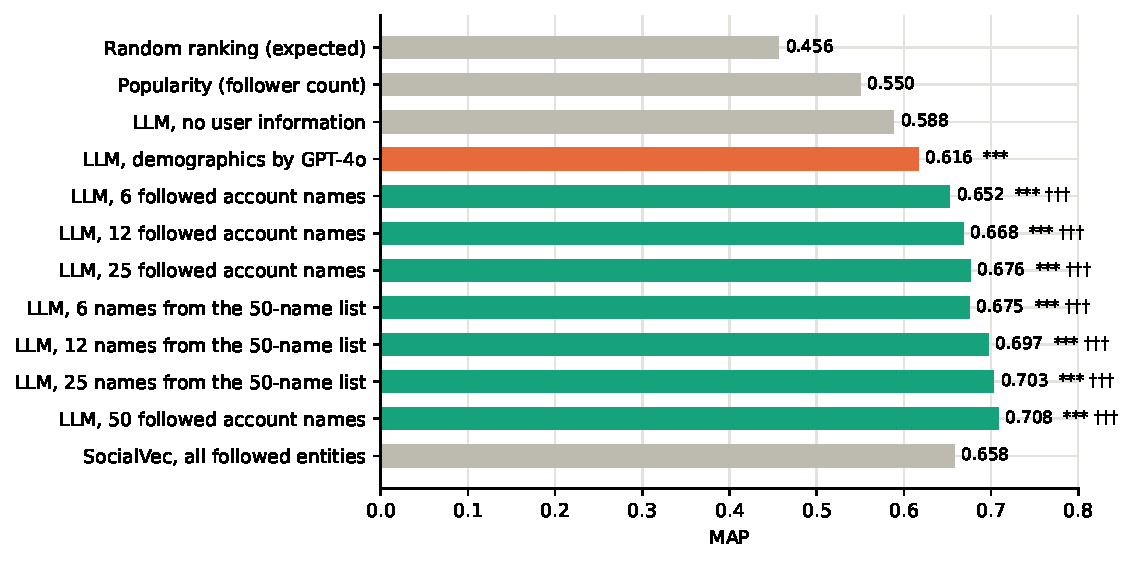
\includegraphics[width=\linewidth,height=0.5\textheight,keepaspectratio]{figures/figure4_ranks_1_20.pdf}
\end{center}

\subsubsection*{Ranks 1--20 \textperiodcentered{} Claude Haiku 5.5 \textperiodcentered{} 1,696 users}
\begin{center}
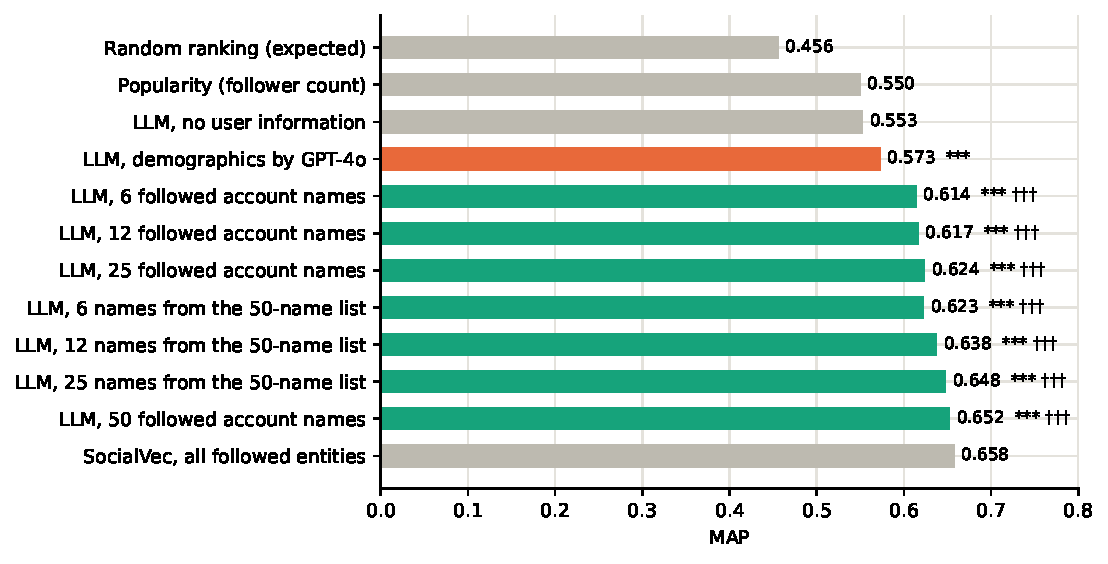
\includegraphics[width=\linewidth,height=0.5\textheight,keepaspectratio]{figures/figure4_ranks_1_20_claude_haiku_5_5.pdf}
\end{center}

\subsubsection*{Ranks 81--100 \textperiodcentered{} GPT-6 Luna \textperiodcentered{} 1,742 users}
\begin{center}
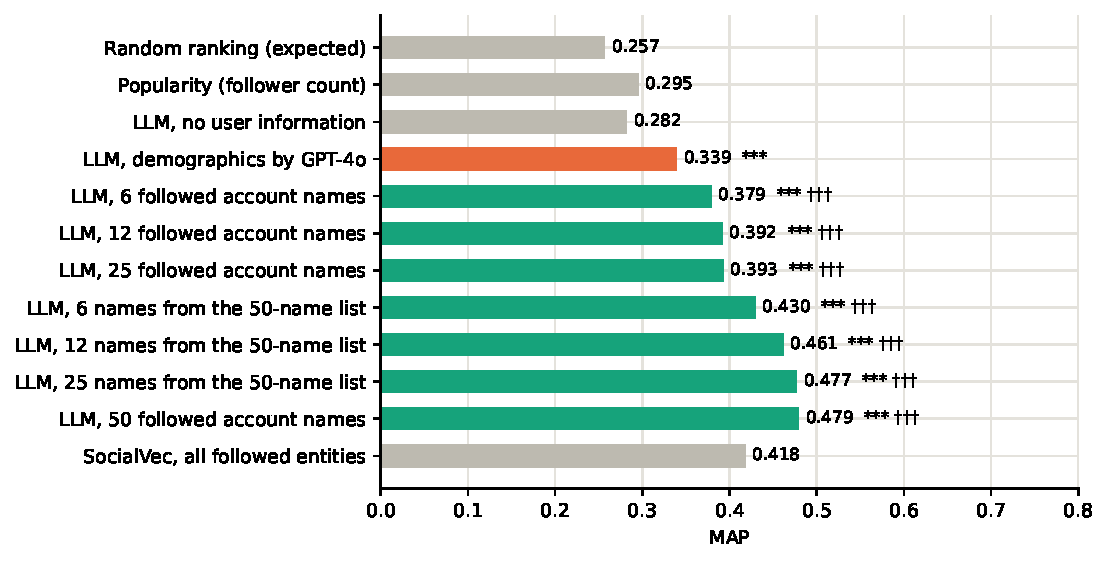
\includegraphics[width=\linewidth,height=0.5\textheight,keepaspectratio]{figures/figure4_ranks_81_100.pdf}
\end{center}

\subsubsection*{Ranks 81--100 \textperiodcentered{} Claude Haiku 5.5 \textperiodcentered{} 1,742 users}
\begin{center}
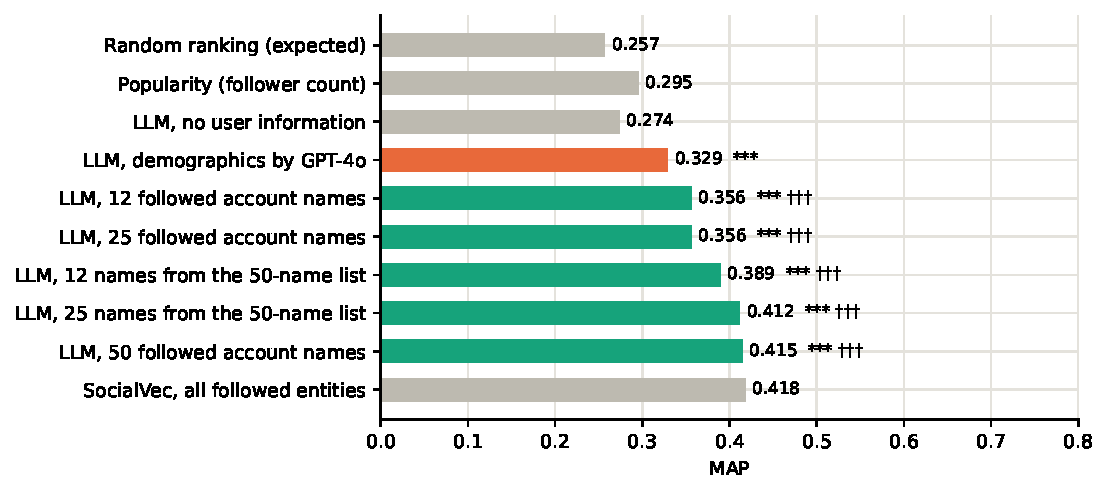
\includegraphics[width=\linewidth,height=0.5\textheight,keepaspectratio]{figures/figure4_ranks_81_100_claude_haiku_5_5.pdf}
\end{center}

{\small Overall MAP (mean over categories) with the candidates in random order. Each band uses the users of Table 15 who follow at least one of its candidates. Markers are paired Wilcoxon tests over users: * vs. the LLM with no user information, \textdagger{} vs. the demographics condition (*/\textdagger{} p \textless{} 0.05, **/\textdagger{}\textdagger{} p \textless{} 0.01, ***/\textdagger{}\textdagger{}\textdagger{} p \textless{} 0.001, n.s. not significant). All but 1 of the 60 comparisons are significant at p \textless{} 0.001; the exception is Claude Haiku 5.5 at ranks 81--100, 6 names vs. demographics (p = 0.014). The p values are in Table 16.}

\subsubsection*{Table 16 \textperiodcentered{} Overall MAP of demographics-only and name-based ranking, ranks 1--20 and 81--100}
\begin{center}\begin{adjustbox}{max width=\linewidth}
\begin{tabular}{lrrrrrr}
\toprule
 & \multicolumn{2}{c}{GPT-6 Luna, all users} & \multicolumn{2}{c}{Claude Haiku 5.5, all users} & \multicolumn{2}{c}{GPT-6 Luna, \textless{} 2,000 follows, $\geq$ 30 entities} \\
Method & Ranks 1--20 & Ranks 81--100 & Ranks 1--20 & Ranks 81--100 & Ranks 1--20 & Ranks 81--100 \\
\midrule
Users & 1,696 & 1,742 & 1,696 & 1,742 & 526 & 533 \\
Random ranking (expected) & 0.456 & 0.257 & 0.456 & 0.257 & 0.474 & 0.247 \\
Popularity (follower count) & 0.550 & 0.295 & 0.550 & 0.295 & 0.600 & 0.287 \\
LLM, no user information & 0.588 & 0.282 & 0.553 & 0.274 & 0.647 & 0.283 \\
LLM, demographics by GPT-4o & 0.616 & 0.339 & 0.573 & 0.329 & 0.659 & 0.350 \\
LLM, 12 followed account names & 0.668 & 0.392 & 0.617 & 0.356 & 0.689 & 0.361 \\
LLM, 25 followed account names & 0.676 & 0.393 & 0.624 & 0.356 & 0.703 & 0.369 \\
LLM, 12 names from the 50-name list & 0.697 & 0.461 & 0.638 & 0.389 & 0.715 & 0.442 \\
LLM, 25 names from the 50-name list & 0.703 & 0.477 & 0.648 & 0.412 & 0.722 & 0.468 \\
LLM, 50 followed account names & 0.708 & 0.479 & 0.652 & 0.415 & 0.735 & 0.473 \\
SocialVec, all followed entities & 0.658 & 0.418 & 0.658 & 0.418 & 0.686 & 0.417 \\
p, demographics vs. no information & \textless{} 0.001 & \textless{} 0.001 & \textless{} 0.001 & \textless{} 0.001 & = 0.209 & \textless{} 0.001 \\
p, 12 names vs. no information & \textless{} 0.001 & \textless{} 0.001 & \textless{} 0.001 & \textless{} 0.001 & \textless{} 0.001 & \textless{} 0.001 \\
p, 25 names vs. no information & \textless{} 0.001 & \textless{} 0.001 & \textless{} 0.001 & \textless{} 0.001 & \textless{} 0.001 & \textless{} 0.001 \\
p, 12 of the 50 names vs. no information & \textless{} 0.001 & \textless{} 0.001 & \textless{} 0.001 & \textless{} 0.001 & \textless{} 0.001 & \textless{} 0.001 \\
p, 25 of the 50 names vs. no information & \textless{} 0.001 & \textless{} 0.001 & \textless{} 0.001 & \textless{} 0.001 & \textless{} 0.001 & \textless{} 0.001 \\
p, 50 names vs. no information & \textless{} 0.001 & \textless{} 0.001 & \textless{} 0.001 & \textless{} 0.001 & \textless{} 0.001 & \textless{} 0.001 \\
p, 12 names vs. demographics & \textless{} 0.001 & \textless{} 0.001 & \textless{} 0.001 & \textless{} 0.001 & \textless{} 0.001 & = 0.225 \\
p, 25 names vs. demographics & \textless{} 0.001 & \textless{} 0.001 & \textless{} 0.001 & \textless{} 0.001 & \textless{} 0.001 & = 0.040 \\
p, 12 of the 50 names vs. demographics & \textless{} 0.001 & \textless{} 0.001 & \textless{} 0.001 & \textless{} 0.001 & \textless{} 0.001 & \textless{} 0.001 \\
p, 25 of the 50 names vs. demographics & \textless{} 0.001 & \textless{} 0.001 & \textless{} 0.001 & \textless{} 0.001 & \textless{} 0.001 & \textless{} 0.001 \\
p, 50 names vs. demographics & \textless{} 0.001 & \textless{} 0.001 & \textless{} 0.001 & \textless{} 0.001 & \textless{} 0.001 & \textless{} 0.001 \\
p, 50 names vs. SocialVec & \textless{} 0.001 & \textless{} 0.001 & = 0.962 & = 0.861 & \textless{} 0.001 & \textless{} 0.001 \\
p, 12 of the 50 names vs. 12 names & \textless{} 0.001 & \textless{} 0.001 & \textless{} 0.001 & \textless{} 0.001 & = 0.005 & \textless{} 0.001 \\
p, 25 of the 50 names vs. 25 names & \textless{} 0.001 & \textless{} 0.001 & \textless{} 0.001 & \textless{} 0.001 & = 0.240 & \textless{} 0.001 \\
p, 50 names vs. 25 of the 50 & = 0.007 & = 0.531 & = 0.100 & = 0.334 & = 0.002 & = 0.306 \\
\bottomrule
\end{tabular}

\end{adjustbox}\end{center}

{\small Overall MAP is the mean over categories; p values are paired Wilcoxon tests over users. The all-users columns are the users of Table 9 (ranks 81--100) and Table 11 (ranks 1--20), with the same random candidate orders, so their no-information, account-name and SocialVec scores are those tables' values.}

\subsection*{Where the account names come from vs. how many there are}
The 12 and 25 names come from the user's closed set (the entities of the other categories' lists the user follows), while the 50 come from everything the user follows. Going from 25 to 50 names therefore changes two things at once: the number of accounts and where they come from. To separate the two, both models also ranked the candidates, in the same candidate order, from names of the full follow list: 25 drawn at random (fixed seed) from the names of the user's k = 50 prompt, the first 12 of those 25 and the first 6 of those 12. A sixth closed-set condition lists the first 6 names of the closed-set k = 12 prompt. Each smaller list is nested in the larger one from the same source. The prompts list 6.0, 11.7 and 21.7 names on average from the closed set, and 6.0, 11.9 and 22.5 from the full follow list (27.9 with k = 50), so each pair of conditions differs in one factor.

\begin{itemize}
  \item \textbf{Where the names come from matters at every size.} At ranks 81--100, names from the full follow list beat closed-set names by +0.051, +0.070 and +0.084 with 6, 12 and 25 names for GPT-6 Luna, and by +0.031, +0.033 and +0.055 for Claude Haiku 5.5: the gap grows with the number of names. At ranks 1--20 it is smaller (+0.009 to +0.028). All these differences are significant except Claude Haiku 5.5 at ranks 1--20 with 6 names (p = 0.053).
  \item \textbf{More closed-set names add little; more names from the full list help up to 25.} From the closed set, 6 $\rightarrow$ 12 names adds +0.003 to +0.016 MAP and 12 $\rightarrow$ 25 adds +0.000 to +0.008 (the k = 25 list of 33\% of users has fewer than 25 names, as they follow fewer closed-set entities). From the full list, 6 $\rightarrow$ 12 adds +0.010 to +0.032, 12 $\rightarrow$ 25 adds +0.006 to +0.022, and 25 $\rightarrow$ 50 only +0.002 to +0.005.
  \item \textbf{So the jump from 25 to 50 names is mostly the change of source:} 97\% of GPT-6 Luna's gain at ranks 81--100 (0.393 $\rightarrow$ 0.479) and 95\% of Claude Haiku 5.5's; 83\% and 84\% at ranks 1--20.
\end{itemize}
For the 38\% of users whose k = 50 prompt lists 25 names or fewer (accounts without a known name are dropped), the 25 names from the 50 are the k = 50 list itself, which is one reason the last step is small.

\subsubsection*{Table 23 \textperiodcentered{} Account names by source and number}
\begin{center}\begin{adjustbox}{max width=\linewidth}
\begin{tabular}{lrrrrrrrrr}
\toprule
 &  &  & \multicolumn{3}{c}{Closed set} & \multicolumn{4}{c}{Full follow list (k = 50 prompt)} \\
Model & Band & Users & 6 & 12 & 25 & 6 & 12 & 25 & 50 \\
\midrule
GPT-6 Luna & Ranks 1--20 & 1,696 & 0.652 & 0.668 & 0.676 & 0.675 & 0.697 & 0.703 & 0.708 \\
GPT-6 Luna & Ranks 81--100 & 1,742 & 0.379 & 0.392 & 0.393 & 0.430 & 0.461 & 0.477 & 0.479 \\
Claude Haiku 5.5 & Ranks 1--20 & 1,696 & 0.614 & 0.617 & 0.624 & 0.623 & 0.638 & 0.648 & 0.652 \\
Claude Haiku 5.5 & Ranks 81--100 & 1,742 & 0.348 & 0.356 & 0.356 & 0.379 & 0.389 & 0.412 & 0.415 \\
\bottomrule
\end{tabular}

\end{adjustbox}\end{center}

{\small Overall MAP (mean over categories). Closed set: the entities of the other categories' lists the user follows (the k = 12 and k = 25 prompts; 6 is the first 6 of the 12). Full follow list: names drawn from the user's k = 50 prompt (25 at random, the first 12 and 6 of those 25, or all of them).}

\subsubsection*{Table 24 \textperiodcentered{} Steps between the account-name conditions}
\begin{center}\begin{adjustbox}{max width=\linewidth}
\begin{tabular}{lrrrrrrrrr}
\toprule
 &  & \multicolumn{3}{c}{Source: full list $-$ closed set} & \multicolumn{5}{c}{Number of names} \\
Model & Band & Source at 6 & Source at 12 & Source at 25 & 6 $\rightarrow$ 12, closed set & 12 $\rightarrow$ 25, closed set & 6 $\rightarrow$ 12, full list & 12 $\rightarrow$ 25, full list & 25 $\rightarrow$ 50, full list \\
\midrule
GPT-6 Luna & Ranks 1--20 & +0.023\newline {\textcolor{gray}{p = 0.001}} & +0.028\newline {\textcolor{gray}{p \textless{} 0.001}} & +0.027\newline {\textcolor{gray}{p \textless{} 0.001}} & +0.016\newline {\textcolor{gray}{p \textless{} 0.001}} & +0.008\newline {\textcolor{gray}{p \textless{} 0.001}} & +0.022\newline {\textcolor{gray}{p \textless{} 0.001}} & +0.006\newline {\textcolor{gray}{p = 0.036}} & +0.005\newline {\textcolor{gray}{p = 0.007}} \\
GPT-6 Luna & Ranks 81--100 & +0.051\newline {\textcolor{gray}{p \textless{} 0.001}} & +0.070\newline {\textcolor{gray}{p \textless{} 0.001}} & +0.084\newline {\textcolor{gray}{p \textless{} 0.001}} & +0.013\newline {\textcolor{gray}{p = 0.002}} & +0.001\newline {\textcolor{gray}{p = 0.523}} & +0.032\newline {\textcolor{gray}{p \textless{} 0.001}} & +0.016\newline {\textcolor{gray}{p = 0.002}} & +0.002\newline {\textcolor{gray}{p = 0.531}} \\
Claude Haiku 5.5 & Ranks 1--20 & +0.009\newline {\textcolor{gray}{p = 0.053}} & +0.021\newline {\textcolor{gray}{p \textless{} 0.001}} & +0.024\newline {\textcolor{gray}{p \textless{} 0.001}} & +0.003\newline {\textcolor{gray}{p = 0.046}} & +0.007\newline {\textcolor{gray}{p = 0.039}} & +0.015\newline {\textcolor{gray}{p \textless{} 0.001}} & +0.010\newline {\textcolor{gray}{p = 0.059}} & +0.004\newline {\textcolor{gray}{p = 0.100}} \\
Claude Haiku 5.5 & Ranks 81--100 & +0.031\newline {\textcolor{gray}{p \textless{} 0.001}} & +0.033\newline {\textcolor{gray}{p \textless{} 0.001}} & +0.055\newline {\textcolor{gray}{p \textless{} 0.001}} & +0.008\newline {\textcolor{gray}{p = 0.058}} & +0.000\newline {\textcolor{gray}{p = 0.980}} & +0.010\newline {\textcolor{gray}{p = 0.031}} & +0.022\newline {\textcolor{gray}{p = 0.003}} & +0.003\newline {\textcolor{gray}{p = 0.334}} \\
\bottomrule
\end{tabular}

\end{adjustbox}\end{center}

{\small The difference in overall MAP between two conditions of Table 23, with the paired Wilcoxon p value over users. Source: the same number of names from the full follow list vs. the closed set. Number of names: the same source, more names.}

\subsection*{What GPT-4o stated about the users}
Each description is parsed with fixed rules for the value it states for each attribute. With the one-value instruction, 84 attribute values across the 1742 descriptions still name more than one value (174 across 270 in the first version); those count under the first value stated. "Middle-aged" is kept as stated, without assigning it an age range.

\begin{itemize}
  \item \textbf{The guesses are concentrated.} 1537 of 1742 descriptions say Caucasian or white and 1642 say higher education without a level. Gender is the most balanced attribute (1019 male, 723 female).
\end{itemize}
\subsubsection*{Figure 5 \textperiodcentered{} Demographic attributes stated in GPT-4o's descriptions \textperiodcentered{} 1742 users}
\begin{center}
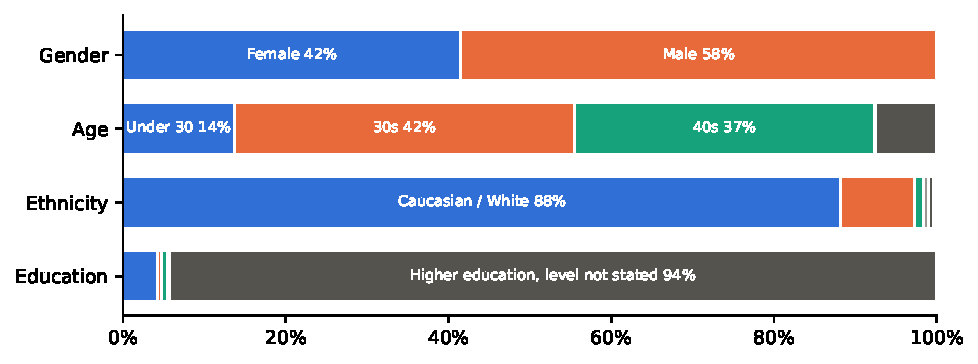
\includegraphics[width=\linewidth,height=0.5\textheight,keepaspectratio]{figures/figure5_attributes.pdf}
\end{center}

{\small Share of descriptions by the value stated for each attribute. Hover a segment for the count.}

\subsection*{Table 17 \textperiodcentered{} Demographic attributes stated in GPT-4o's descriptions}
\begin{center}\begin{adjustbox}{max width=\linewidth}
\begin{tabular}{lrrr}
\toprule
Attribute & First stated value & Descriptions & Share \\
\midrule
Gender & Female & 723 & 42\% \\
 & Male & 1019 & 58\% \\
Age & Under 30 & 238 & 14\% \\
 & 30s & 728 & 42\% \\
 & 40s & 642 & 37\% \\
 & Middle-aged & 2 & 0\% \\
 & 50 or older & 132 & 8\% \\
Ethnicity & Caucasian / White & 1537 & 88\% \\
 & African American / Black & 158 & 9\% \\
 & Hispanic / Latino & 19 & 1\% \\
 & Asian & 11 & 1\% \\
 & Mixed / diverse & 11 & 1\% \\
 & Not stated & 6 & 0\% \\
Education & High school & 73 & 4\% \\
 & Some higher education & 9 & 1\% \\
 & College / university degree & 13 & 1\% \\
 & Graduate degree & 4 & 0\% \\
 & Higher education, level not stated & 1642 & 94\% \\
 & Not stated & 1 & 0\% \\
\bottomrule
\end{tabular}

\end{adjustbox}\end{center}

{\small Education counts a specific level (high school, some higher education, a degree) when one is stated anywhere in the description, and "level not stated" otherwise.}

\subsection*{Table 18 \textperiodcentered{} Demographic attributes stated in GPT-4o's descriptions, by category}
\begin{center}\begin{adjustbox}{max width=\linewidth}
\begin{tabular}{lrrrrrrrrrr}
\toprule
 & \multicolumn{2}{c}{Gender} & \multicolumn{4}{c}{Age} & \multicolumn{2}{c}{Ethnicity} & \multicolumn{2}{c}{Education} \\
Category & Female & Male & Under 30 & 30s & 40s & 50 or older & Caucasian / White & African American / Black & High school & Higher education \\
\midrule
Musical artists & 45\% & 55\% & 41\% & 36\% & 20\% & 3\% & 62\% & 29\% & 11\% & 88\% \\
News outlets & 33\% & 67\% & 4\% & 37\% & 47\% & 12\% & 93\% & 6\% & 2\% & 97\% \\
Comedians & 52\% & 48\% & 6\% & 43\% & 43\% & 7\% & 92\% & 5\% & 1\% & 97\% \\
Politicians & 54\% & 46\% & 5\% & 36\% & 48\% & 11\% & 92\% & 6\% & 1\% & 98\% \\
TV stations & 38\% & 62\% & 11\% & 47\% & 36\% & 6\% & 92\% & 6\% & 5\% & 94\% \\
Actors & 43\% & 57\% & 13\% & 43\% & 36\% & 7\% & 90\% & 8\% & 4\% & 95\% \\
TV shows & 43\% & 57\% & 12\% & 44\% & 38\% & 5\% & 89\% & 9\% & 4\% & 95\% \\
Sports teams & 12\% & 88\% & 32\% & 57\% & 10\% & 1\% & 89\% & 8\% & 10\% & 86\% \\
Journalists & 54\% & 46\% & 0\% & 32\% & 52\% & 16\% & 95\% & 5\% & 1\% & 98\% \\
\midrule
Overall & 42\% & 58\% & 14\% & 42\% & 37\% & 8\% & 88\% & 9\% & 4\% & 94\% \\
\bottomrule
\end{tabular}

\end{adjustbox}\end{center}

{\small Share of the category's descriptions stating each value. Age shows every age group the descriptions use (under 30, 30s, 40s and 50 or older); "middle-aged" appears in only 2 descriptions and is left out; for ethnicity and education only the two most frequent values are shown, and the rest are in Table 17.}

\subsection*{Table 19 \textperiodcentered{} Examples: known entities a user follows and GPT-4o's description}
One user from each of 4 categories: the user whose list of account names (the input to GPT-4o) contains the most known entities, i.e. accounts in the original or extended category lists. The table shows those known entities by name, in the order GPT-4o saw them; GPT-4o also saw the user's other, less known accounts (the "Known / all" column), and the description is the one it wrote from the full list. No model was called again for these examples. Possible motivating examples.

\begin{center}\begin{adjustbox}{max width=\linewidth}
\begin{tabular}{lp{0.38\linewidth}rp{0.38\linewidth}}
\toprule
Sampled for & Known entities among the accounts GPT-4o saw & Known / all & GPT-4o's description \\
\midrule
Musical artists & Shia LaBeouf, Shanola Hampton, Ellie Goulding, Mehdi Hasan, Dave Coulier, Gillian Anderson, Nina Dobrev, Blake Lively, billy eichner, San Francisco 49ers, Dave Mustaine, Channing Tatum, Jimmy Kimmel, pw, Lamorne Morris, Keegan Allen, Michael Keaton, terry crews, Elizabeth Spiers, John Kasich, Kelly!, Mr. T, IT'S CHRISTMAS TIME, Phreddie Prinze Jr., Joyce Alene, Seth Rogen, Brody Jenner, Jamie Lynn Spears, Good Morning America & 29 of 44 & The user is most likely a Caucasian male in his 30s with a higher education level. \\
Sports teams & Joel McHale, Animal Planet, Tay Zonday, Kristen Bell, iamcardib, Kevin Hart, Melissa McCarthy, Jackée Harry, Wendy's, Jimmy Kimmel, Eva Longoria Baston, Seth Meyers, Melissa McBride, Ariana Grande, TMZ, Jimmy Kimmel Live, daniel tosh, Bindi Irwin, Wanda Sykes, Conan O'Brien & 20 of 40 & The user is most likely a Caucasian male in their 30s with higher education. \\
Politicians & Ice-T, CNN Breaking News, Rickey Smiley, Ari Melber, Bill Maher, Yamiche Alcindor, Sunny Hostin, Rihanna, Ellen DeGeneres, Jill Scott, Steve Schmidt, Anderson Cooper 360, Rachel Maddow MSNBC, Joy Reid, Leslie Jones, Don Lemon, Tiffany Cross, Maya Wiley, Elie Mystal, P!nk, Joe Scarborough, Tish James, AprilDRyan, A N G E L A | R Y E, Whoopi Goldberg, BEYONCÉ, Meek Mill, Ashley Nicole Black, Stephen Colbert, Kandi Burruss, Symone D. Sanders, Jim Acosta, iamcardib & 33 of 42 & The user is most likely a Black female in their 30s with higher education. \\
News outlets & Preet Bharara, Clarissa Ward, Joe Walsh, Fran Drescher, Jonathan Lemire, Pete Buttigieg, Kamala Harris, CookPoliticalReport, Katie Couric, Governor Gretchen Whitmer, Brooke Baldwin, Kate Bolduan, Chaz Bono, Gabrielle Giffords, Mimi Rocah, The Hill, The View, ashley judd, Karine Jean-Pierre, Bill Clinton, Dan Rather, Chuck Schumer, Ilhan Omar, Taylor Swift & 24 of 43 & The user is most likely a Caucasian female in her 50s with higher education. \\
\bottomrule
\end{tabular}

\end{adjustbox}\end{center}

{\small The descriptions are stereotype-based guesses about real people, shown here identified only by category. They should not be read as findings about which groups like which entities.}

\section*{S\quad Supplementary \textperiodcentered{} Ranking with Claude Haiku 5.5}
All results of the Claude Haiku 5.5 rankings of Section 5: the same 1,742 users (ranks 81--100) and 1,696 users (ranks 1--20), candidate orders, GPT-4o descriptions and prompts as GPT-6 Luna.

Claude Haiku 5.5 received the exact chat messages dspy renders for each signature (system and user message), through the Anthropic API with adaptive thinking at effort \emph{low} and the Message Batches API: 31,941 calls costing \$3.91. The answer's \texttt{ranked\_ids} field is scored as for GPT-6 Luna: candidates it leaves out count as misses. The overall figures are in Table 16 and Figure 4.

\subsection*{Table 20 \textperiodcentered{} Supplementary \textperiodcentered{} Claude Haiku 5.5 ranking per category, ranks 1--20}
\begin{center}\begin{adjustbox}{max width=\linewidth}
\begin{tabular}{lrrrrrrrrrrrrr}
\toprule
 &  & \multicolumn{2}{c}{Non-personalized} & SocialVec & \multicolumn{5}{c}{Claude Haiku 5.5} \\
Category & Users & Random & Popularity & All entities & No user information & Demographics by GPT-4o & 6 account names & 12 account names & 25 account names & 6 names from the 50 & 12 names from the 50 & 25 names from the 50 & 50 account names \\
\midrule
Musical artists & 183 & 0.460 & 0.564 & \textbf{0.668} & 0.552 & 0.609 & 0.572 & 0.560 & 0.566 & 0.586 & 0.599 & 0.603 & 0.614 \\
News outlets & 186 & 0.512 & 0.616 & 0.694 & 0.617 & 0.616 & 0.679 & 0.695 & 0.707 & 0.694 & 0.703 & 0.721 & \textbf{0.721} \\
Comedians & 197 & 0.522 & 0.612 & 0.675 & 0.612 & 0.618 & 0.685 & \textbf{0.694} & 0.692 & 0.671 & 0.682 & 0.691 & 0.687 \\
Politicians & 195 & 0.565 & 0.662 & 0.706 & 0.707 & 0.704 & 0.732 & 0.734 & 0.740 & 0.724 & 0.748 & \textbf{0.750} & 0.745 \\
TV stations & 187 & 0.389 & 0.575 & 0.653 & 0.584 & 0.588 & 0.630 & 0.666 & 0.686 & 0.643 & 0.666 & \textbf{0.689} & 0.682 \\
Actors & 185 & 0.437 & 0.481 & \textbf{0.620} & 0.531 & 0.575 & 0.519 & 0.493 & 0.501 & 0.562 & 0.547 & 0.552 & 0.570 \\
TV shows & 187 & 0.293 & 0.450 & \textbf{0.628} & 0.418 & 0.429 & 0.616 & 0.609 & 0.620 & 0.559 & 0.579 & 0.591 & 0.598 \\
Sports teams & 184 & 0.395 & 0.413 & \textbf{0.600} & 0.399 & 0.443 & 0.465 & 0.447 & 0.456 & 0.518 & 0.567 & 0.573 & 0.587 \\
Journalists & 192 & 0.534 & 0.577 & \textbf{0.675} & 0.553 & 0.575 & 0.628 & 0.653 & 0.647 & 0.647 & 0.649 & 0.661 & 0.667 \\
\midrule
Overall & 1,696 & 0.456 & 0.550 & \textbf{0.658} & 0.553 & 0.573 & 0.614 & 0.617 & 0.624 & 0.623 & 0.638 & 0.648 & 0.652 \\
GPT-6 Luna, overall &  &  &  &  & 0.588 & 0.616 & 0.652 & 0.668 & 0.676 & 0.675 & 0.697 & 0.703 & 0.708 \\
\bottomrule
\end{tabular}

\end{adjustbox}\end{center}

{\small MAP per category with the candidates in each user's random order; Overall is the mean over categories. Bold marks the best method in each row. The last row gives GPT-6 Luna's overall MAP in the same conditions (Table 16).}

\subsection*{Table 21 \textperiodcentered{} Supplementary \textperiodcentered{} Claude Haiku 5.5 ranking per category, ranks 81--100}
\begin{center}\begin{adjustbox}{max width=\linewidth}
\begin{tabular}{lrrrrrrrrrrrrr}
\toprule
 &  & \multicolumn{2}{c}{Non-personalized} & SocialVec & \multicolumn{5}{c}{Claude Haiku 5.5} \\
Category & Users & Random & Popularity & All entities & No user information & Demographics by GPT-4o & 6 account names & 12 account names & 25 account names & 6 names from the 50 & 12 names from the 50 & 25 names from the 50 & 50 account names \\
\midrule
Musical artists & 196 & 0.240 & 0.345 & \textbf{0.528} & 0.231 & 0.376 & 0.270 & 0.301 & 0.300 & 0.341 & 0.369 & 0.396 & 0.403 \\
News outlets & 189 & 0.241 & 0.215 & 0.382 & 0.267 & 0.304 & 0.399 & 0.407 & \textbf{0.412} & 0.400 & 0.380 & 0.412 & 0.399 \\
Comedians & 198 & 0.213 & \textbf{0.371} & 0.271 & 0.225 & 0.217 & 0.277 & 0.289 & 0.287 & 0.240 & 0.256 & 0.282 & 0.285 \\
Politicians & 196 & 0.369 & 0.347 & 0.454 & 0.369 & 0.429 & 0.453 & 0.488 & 0.484 & 0.482 & 0.487 & 0.493 & \textbf{0.507} \\
TV stations & 189 & 0.197 & 0.186 & 0.414 & 0.225 & 0.245 & 0.299 & 0.298 & 0.312 & 0.391 & 0.402 & 0.444 & \textbf{0.474} \\
Actors & 198 & 0.272 & 0.309 & \textbf{0.480} & 0.272 & 0.350 & 0.371 & 0.390 & 0.367 & 0.401 & 0.415 & 0.436 & 0.444 \\
TV shows & 192 & 0.215 & 0.334 & \textbf{0.396} & 0.250 & 0.339 & 0.346 & 0.326 & 0.333 & 0.340 & 0.339 & 0.389 & 0.372 \\
Sports teams & 190 & 0.245 & 0.255 & \textbf{0.445} & 0.288 & 0.328 & 0.317 & 0.312 & 0.314 & 0.416 & 0.419 & 0.424 & 0.433 \\
Journalists & 194 & 0.321 & 0.295 & 0.392 & 0.335 & 0.374 & 0.402 & 0.395 & 0.398 & 0.404 & \textbf{0.437} & 0.429 & 0.417 \\
\midrule
Overall & 1,742 & 0.257 & 0.295 & \textbf{0.418} & 0.274 & 0.329 & 0.348 & 0.356 & 0.356 & 0.379 & 0.389 & 0.412 & 0.415 \\
GPT-6 Luna, overall &  &  &  &  & 0.282 & 0.339 & 0.379 & 0.392 & 0.393 & 0.430 & 0.461 & 0.477 & 0.479 \\
\bottomrule
\end{tabular}

\end{adjustbox}\end{center}

{\small As above, for the candidates at ranks 81--100.}

\subsection*{Table 22 \textperiodcentered{} Supplementary \textperiodcentered{} Completeness of the rankings, Claude Haiku 5.5 and GPT-6 Luna}
\begin{center}\begin{adjustbox}{max width=\linewidth}
\begin{tabular}{lrrrrrrrrrrrrrrrrrrrrrr}
\toprule
 &  & \multicolumn{3}{c}{No user information} & \multicolumn{3}{c}{Demographics by GPT-4o} & \multicolumn{3}{c}{12 account names} & \multicolumn{3}{c}{25 account names} & \multicolumn{3}{c}{12 names from the 50} & \multicolumn{3}{c}{25 names from the 50} & \multicolumn{3}{c}{50 account names} \\
Model & Band & All & $\geq$ 95\% & None & All & $\geq$ 95\% & None & All & $\geq$ 95\% & None & All & $\geq$ 95\% & None & All & $\geq$ 95\% & None & All & $\geq$ 95\% & None & All & $\geq$ 95\% & None \\
\midrule
Claude Haiku 5.5 & Ranks 1--20 & 99.5\% & 99.8\% & 0.0\% & 98.9\% & 99.7\% & 0.1\% & 98.8\% & 99.8\% & 0.1\% & 97.8\% & 99.9\% & 0.1\% & 98.8\% & 99.9\% & 0.1\% & 97.9\% & 99.5\% & 0.3\% & 97.3\% & 99.7\% & 0.2\% \\
Claude Haiku 5.5 & Ranks 81--100 & 99.7\% & 99.9\% & 0.1\% & 99.1\% & 99.5\% & 0.3\% & 98.4\% & 99.2\% & 0.2\% & 98.2\% & 99.3\% & 0.3\% & 98.1\% & 99.3\% & 0.2\% & 98.0\% & 99.2\% & 0.2\% & 97.9\% & 99.2\% & 0.2\% \\
GPT-6 Luna & Ranks 1--20 & 96.3\% & 99.9\% & 0.0\% & 90.8\% & 98.9\% & 0.0\% & 84.6\% & 98.2\% & 0.0\% & 84.0\% & 98.3\% & 0.0\% & 83.0\% & 99.1\% & 0.0\% & 86.0\% & 98.8\% & 0.0\% & 86.0\% & 98.6\% & 0.1\% \\
GPT-6 Luna & Ranks 81--100 & 97.0\% & 99.1\% & 0.0\% & 92.5\% & 97.4\% & 0.0\% & 86.6\% & 96.6\% & 0.0\% & 88.2\% & 97.5\% & 0.1\% & 83.5\% & 95.2\% & 0.1\% & 86.7\% & 96.7\% & 0.1\% & 88.1\% & 97.5\% & 0.1\% \\
\bottomrule
\end{tabular}

\end{adjustbox}\end{center}

{\small Share of answers whose \texttt{ranked\_ids} contain every candidate, at least 95\% of them, or no usable ranking at all, per model, band and condition.}

\section{Open items}
\noindent\textsc{scale}\par
\subsubsection*{LLM experiments on all users}
The LLM results still use samples: 50 users per category for Table 3 (700 of the 11,153 users), and 200 per category for Table 9--Table 11, Section 5 and the supplement (1,742 of the 3,798 users who follow a ranks 81--100 candidate; TV stations have only 198). Overall MAP is then within about $\pm$0.01. Running every remaining user would take about 73K more calls, about \$19 at this page's measured cost per call: Table 3 \textasciitilde{}31K calls (\textasciitilde{}\$8), Table 9--Table 11 \textasciitilde{}16K (\textasciitilde{}\$4), Section 5 \textasciitilde{}6K (\textasciitilde{}\$4, with the GPT-4o descriptions), Claude Haiku 5.5 \textasciitilde{}20K (\textasciitilde{}\$2). The same scripts run larger samples, and cached responses are reused.

\noindent\textsc{next}\par
\subsubsection*{Description-based tail candidates}
The requested variant selects 50--100 accounts per category by their \emph{textual descriptions}, below the top 10K/20K SocialVec entities. The ranks 81--100 band does not meet that criterion fully: 110 of its 177 candidates (62\%) fall below the top 10K, and it uses the typed lists rather than descriptions.

\section*{About these results}
Regenerate the underlying results with \texttt{python run\_reproduction.py}, \texttt{python run\_popularity\_band.py --start 81 --end 100} and \texttt{python run\_llm\_experiments.py}. For Section 5, run \texttt{python run\_llm\_demographics.py} (with \texttt{--describe-model gpt-4o} for the repeat), \texttt{python run\_llm\_demographics\_bands.py} and \texttt{python make\_demographics\_report.py}. Then rebuild this page with \texttt{python make\_results\_page.py}. Details are in \texttt{results/REPORT.md}, \texttt{results/POPULARITY\_BAND\_REPORT.md} and \texttt{results/LLM\_REPORT.md}. Results that use the extended category lists are kept in results\_backup.html.

\end{document}
